%% ----------------------------------------------------------------
%% Project.tex
%% ----------------------------------------------------------------
\documentclass[sotoncolour]{extra/uos_project}     % Use the Project Style with custom link colour
\usepackage[round]{natbib}           % Use Natbib style for the refs.
\usepackage{bibentry}                % Use bibentry for prepublished works
\usepackage{pdfpages}                % Use pdfpages to enables pdf's to be inserted into the project
\usepackage{wrapfig}                 % Use wrapfig for wrapped figures
\usepackage{float}                   % Use for locating figure and table locations
\usepackage{verbatim}                % use for word count
\usepackage{attrib}                  % Use the attrib package for quotations

\nobibliography*                     % Use bibentry for prepublished works
\hypersetup{colorlinks=true}         % Set to false for black/white printing
%% ----------------------------------------------------------------
%% Definitions.tex
%% ----------------------------------------------------------------
\newcommand{\BibTeX}{{\rm B\kern-.05em{\sc i\kern-.025em b}\kern-.08em T\kern-.1667em\lower.7ex\hbox{E}\kern-.125emX}}

%% People
\newcounter{address}
\setcounter{address}{1}
\renewcommand{\theaddress}{\textsuperscript{\fnsymbol{address}}}
\newcommand{\address}[1]{\refstepcounter{address}\theaddress#1\\}
\newcommand{\Name}[3]{\texorpdfstring{\href{mailto:#3}{#2}#1}{#2}\xspace}
\newcommand{\SteveRGunn}[1]{\Name{#1}{Steve R. Gunn}{S.R.Gunn@ecs.soton.ac.uk}}

%% Dingbats
\newcommand{\tick}{\ding{51}}
\newcommand{\cross}{\ding{55}}

%% Calculus
\newcommand{\pd}[2]{\ensuremath{\frac{\partial #1}{\partial #2}}\xspace}
\newcommand{\fd}[2]{\ensuremath{\frac{d #1}{d #2}}\xspace}
\newcommand{\dint}{\ensuremath{\int\!\!\!\int}\xspace}
\newcommand{\tint}{\ensuremath{\int\!\!\!\int\!\!\!\int}\xspace}

%% Math Sets
\newcommand{\Q}[1]{\ensuremath{\mathbb{#1}}\xspace}
\newcommand{\R}{\Q{R}}

%% Matrix, Vector
\newcommand{\V}[1]{\ensuremath{\boldsymbol{#1}}\xspace}
\newcommand{\M}[1]{\ensuremath{\boldsymbol{#1}}\xspace}
\newcommand{\0}{\V{0}}
\newcommand{\1}{\V{1}}
\newcommand{\I}{\M{I}}

%% Math Functions
\newcommand{\F}[1]{\ensuremath{\mathrm{#1}}\xspace}
\newcommand{\sgn}{\F{sgn}}
\newcommand{\tr}{\F{trace}}
\newcommand{\diag}{\F{diag}}

%% Math Names
\newcommand{\N}[1]{\ensuremath{\mathit{#1}}\xspace}

%% Data
\newcommand{\mc}[1]{\ensuremath{\mathcal{#1}}\xspace}
\newcommand{\Hyp}{\mc{H}}
\newcommand{\D}{\mc{D}}

%% Kernel
\newcommand{\K}{\M{K}}
\newcommand{\eins}{\texorpdfstring{\ensuremath{\epsilon}}{\textepsilon}-insensitive\xspace}
\newcommand{\e}{\ensuremath{\epsilon}\xspace}
\newcommand{\Bxi}{\ensuremath{\boldsymbol{\xi}}\xspace}
\newcommand{\Kanova}{\ensuremath{\mathit{K_{ANOVA}}}\xspace}
\newcommand{\Kspline}{\ensuremath{\mathit{K_{spline}}}\xspace}

%% Bayesian
\newcommand{\MP}{\ensuremath{\mathit{{\scriptscriptstyle \hspace{-1.5pt}M\hspace{-1.5pt}P}}}\xspace}
\newcommand{\ML}{\ensuremath{\mathit{{\scriptscriptstyle \hspace{-1.5pt}M\hspace{-1.5pt}L}}}\xspace}
\newcommand{\Qw}{\ensuremath{Q_{\w}(\w)}\xspace}
\newcommand{\Qa}{\ensuremath{Q_{\Ba}(\Ba)}\xspace}
\newcommand{\Qb}{\ensuremath{Q_{\beta}(\beta)}\xspace}
\newcommand{\wMPab}{\ensuremath{\w_{\MP|\bar {\Ba},\bar \beta}}\xspace}
\newcommand{\wMP}{\ensuremath{\w_{\MP}}\xspace}
\newcommand{\yMP}{\ensuremath{y_{\MP}}\xspace}
\newcommand{\BaMP}{\ensuremath{\Ba_{\hspace{1pt}\MP}}\xspace}
\newcommand{\aMP}{\ensuremath{\alpha_{\hspace{1pt}\MP}}\xspace}
\newcommand{\bMP}{\ensuremath{\beta_{\hspace{1pt}\MP}}\xspace}
\newcommand{\Sab}{\ensuremath{\M{\Sigma}_{\bar \Ba,\bar \beta}}\xspace}
\newcommand{\Ba}{\ensuremath{\boldsymbol{\alpha}}\xspace}
\newcommand{\Bb}{\ensuremath{\boldsymbol{\beta}}\xspace}
\newcommand{\Bm}{\ensuremath{\boldsymbol{\mu}}\xspace}
\newcommand{\BL}{\ensuremath{\boldsymbol{\Lambda}}\xspace}
\newcommand{\BPhi}{\ensuremath{\boldsymbol{\Phi}}\xspace}
\newcommand{\SMP}{\ensuremath{\M{\Sigma}_{\MP}}\xspace}

\newcommand{\Pa}{\ensuremath{P(\alpha|\mathcal{H})}\xspace}
\newcommand{\Pb}{\ensuremath{P(\beta|\mathcal{H})}\xspace}
\newcommand{\Pab}{\ensuremath{P(\alpha,\beta|\mathcal{H})}\xspace}
\newcommand{\Pw}{\ensuremath{P(\w|\mathcal{H})}\xspace}
\newcommand{\PD}{\ensuremath{P(\D|\mathcal{H})}\xspace}
\newcommand{\PwIa}{\ensuremath{P(\w|\alpha,\mathcal{H})}\xspace}
\newcommand{\PDIwb}{\ensuremath{P(\D|\w,\beta,\mathcal{H})}\xspace}
\newcommand{\PDwab}{\ensuremath{P(\D,\w,\alpha,\beta|\mathcal{H})}\xspace}
\newcommand{\PDIw}{\ensuremath{P(\D|\w,\mathcal{H})}\xspace}
\newcommand{\PwID}{\ensuremath{P(\w|\D,\mathcal{H})}\xspace}
\newcommand{\PwabID}{\ensuremath{P(\w,\alpha,\beta|\D,\mathcal{H})}\xspace}

\newcommand{\PanH}{\ensuremath{P(\alpha)}\xspace}
\newcommand{\PbnH}{\ensuremath{P(\beta)}\xspace}
\newcommand{\PabnH}{\ensuremath{P(\alpha,\beta)}\xspace}
\newcommand{\PwnH}{\ensuremath{P(\w)}\xspace}
\newcommand{\PDnH}{\ensuremath{P(\D)}\xspace}
\newcommand{\PwIanH}{\ensuremath{P(\w|\alpha)}\xspace}
\newcommand{\PDIwbnH}{\ensuremath{P(\D|\w,\beta)}\xspace}
\newcommand{\PDwabnH}{\ensuremath{P(\D,\w,\Ba,\beta)}\xspace}
\newcommand{\PDIwnH}{\ensuremath{P(\D|\w)}\xspace}
\newcommand{\PwIDnH}{\ensuremath{P(\w|\D)}\xspace}
\newcommand{\PwabIDnH}{\ensuremath{P(\w,\alpha,\beta|\D)}\xspace}

\newcommand{\PDwBab}{\ensuremath{P(\D,\w,\Ba,\beta|\mathcal{H})}\xspace}
\newcommand{\PwIBa}{\ensuremath{P(\w|\Ba,\mathcal{H})}\xspace}
\newcommand{\PBab}{\ensuremath{P(\Ba,\beta|\mathcal{H})}\xspace}
\newcommand{\PwBabID}{\ensuremath{P(\w,\Ba,\beta|\D,\mathcal{H})}\xspace}

\newcommand{\PBanH}{\ensuremath{P(\Ba)}\xspace}
\newcommand{\PwIBanH}{\ensuremath{P(\w|\Ba)}\xspace}

%% Snakes
\newcommand{\Esnake}{\ensuremath{\mathit{E_{snake}}}\xspace}
\newcommand{\Eimage}{\ensuremath{\mathit{E_{image}}}\xspace}
\newcommand{\Econt}{\ensuremath{\mathit{E_{cont}}}\xspace}
\newcommand{\Ecurv}{\ensuremath{\mathit{E_{curv}}}\xspace}
\newcommand{\Eint}{\ensuremath{\mathit{E_{int}}}\xspace}
\newcommand{\Eext}{\ensuremath{\mathit{E_{ext}}}\xspace}
\newcommand{\Eterm}{\ensuremath{\mathit{E_{term}}}\xspace}
\newcommand{\Eline}{\ensuremath{\mathit{E_{line}}}\xspace}
\newcommand{\Eedge}{\ensuremath{\mathit{E_{edge}}}\xspace}
\newcommand{\Econ}{\ensuremath{\mathit{E_{con}}}\xspace}
\newcommand{\Eangle}{\ensuremath{\mathit{E_{angle}}}\xspace}
\newcommand{\Elshape}{\ensuremath{\mathit{E_{lshape}}}\xspace}
\newcommand{\Eedgedir}{\ensuremath{\mathit{E_{edgedir}}}\xspace}
\newcommand{\Emodel}{\ensuremath{\mathit{E_{model}}}\xspace}
\newcommand{\wte}{\ensuremath{\mathit{w_{term}}}\xspace}
\newcommand{\wli}{\ensuremath{\mathit{w_{line}}}\xspace}
\newcommand{\wed}{\ensuremath{\mathit{w_{edge}}}\xspace}
\newcommand{\wco}{\ensuremath{\mathit{w_{con}}}\xspace}

%% Environments
\newcounter{alg}
\newenvironment{algorithm}[1]
{
    \stepcounter{alg}
    \begin{table}[htb]
    \centering
    \begin{tabular}[t]{ll}
    \hline&\\
    \multicolumn{2}{l}{\bf Algorithm \arabic{alg}: #1}\\&\\
} {
    &\\
    \hline
    \end{tabular}
    \end{table}
}
            % Include your abbreviations
\pdfminorversion=7                   % Fixes warnings for importing pdf documents
\newcommand\wordcount{\verbatiminput{extra/wordcount.sum}}  % For word count command in appendix

\hyphenpenalty=10000
\tolerance=5000
\emergencystretch=2.5em

\lstloadlanguages{Python}  % Used for lstlisting
\lstset{
  language=Python,
  basicstyle=\scriptsize\sffamily,
  numberstyle=\color{gray},
  stringstyle=\color[HTML]{933797},
  commentstyle=\color[HTML]{228B22}\sffamily,
  emph={[2]from,import,pass,return}, emphstyle={[2]\color[HTML]{DD52F0}},
  emph={[3]range}, emphstyle={[3]\color[HTML]{D17032}},
  emph={[4]for,in,def}, emphstyle={[4]\color{blue}},
  showstringspaces=false,
  breaklines=true,
  prebreak=\mbox{{\color{gray}\tiny$\searrow$}},
  numbers=left,
  xleftmargin=15pt,
  aboveskip=10pt
}

%% ----------------------------------------------------------------
%% --------------------THESIS/DOC INFORMATION ---------------------
\department  {School of Electronics and Computer Science}
\DEPARTMENT  {\MakeUppercase{\deptname}}
\group       {}
\GROUP       {\MakeUppercase{\groupname}}
\faculty     {Faculty of Physical Engineering and Science}
\FACULTY     {\MakeUppercase{\facname}}
\title       {Reinforcement Learning agents for Online Elastic Resource allocation in Mobile Edge Computing}
\authors     {\texorpdfstring
             {\href{mailto:mt5g17@soton.ac.uk}{Mark Towers}}
             {Mark Towers}}
\addresses  {\groupname\\\deptname\\\univname}
\date       {\today}
\supervisor {Dr Timothy Norman}
\examiner   {Dr Nicholas Harris}
\degree     {MEng Computer Science}
%% \qualifications{}
\subject    {}
\keywords   {Edge Cloud Computing, Auctions, Resource Allocation, Reinforcement Learning}

\begin{document}
%% ------------------ FRONT MATTER ORGANISATION -------------------
\frontmatter
\maketitle
\begin{abstract}
Mobile Edge clouds enable computational tasks to be completed at the edge of the network, without relying on access to
remote data centres. A key challenge in these settings is that servers have limited computational resources that often
need to be allocated to many self-interested users. Existing resource allocation approaches usually assume that tasks
have inelastic resource requirements (i.e., a fixed amount of computation, bandwidth and storage), which may result in
inefficient resource use and even bottlenecks. In this project, an elastic resource requirement mechanism is expanded
upon to an online setting, such that tasks arrive over time with the prices and resource allocation determined by
agents trained using reinforcement learning.
\end{abstract}

\pdfbookmark[0]{\contentsname}{toc}
\tableofcontents
\listoffigures
\listoftables
%% The List of listings does not, by default, appear in the ToC, so....
\addtotoc{Listings}
% \lstlistoflistings
% \listofaddmaterial
% \addtolom{Material Name e.g Map}
% \addtolom{Material Name e.g CD}
% \addtolom{Test Material}

%% ---------- AUTHORSHIP DECLARATION/ ACKNOW. / DEDICATORY ----------
%% Either include citations like below (as many as required spaced with commas or 'and').
%% \bibentry command must be used here with prepublished papers
\authorshipdeclaration{\bibentry{Gunn:2001:pdflatex}\newline\bibentry{Lovell:2011:updated}\newline\bibentry{Gunn:2011:updated2}}
%% Or state no citations like below
%% \authorshipdeclaration{}
%% -----------------------
\acknowledgements{
  I want to thank my family (especially Maggie, the cat) for all their support over the years as I would not be where I
  am now without them. \\
  To my housemates for surviving with me pestering them about proof reading badly written papers and for dealing with me
  stressing about this project.

  This project wouldn't have started without Dr Sebastian Stein, Professor Tim Norman and a team of Pennsylvania State
  University that has produced a paper investigating the static case of this problem. Thank to all of them for sharing
  ideas and support for that paper and this project. \\
  To Professor Timothy Norman for this constant guidance over the project and for surviving my bad spelling and grammar.
}

\mainmatter
%% ------------------ MAIN MATTER (CONTENT) --------------------
\chapter{Introduction}\label{ch:project-problem}
Cloud computing is a rapidly growing technology with competition from Google, Amazon, Microsoft and others that aims to
allow users to run computer programs that are too large, difficult or time consuming to run locally.
These services provide the computational resources, e.g.\ CPU cores, RAM, hard drive space, bandwidth, etc
to be able to run such programs. However, as these resources are limited, if users request an unbalance quantity of
resources, bottlenecks can occur limiting the number of tasks~\footnote{Tasks, Programs and Jobs will be used
interchangeable to refer to the same idea of a computer programs that has a fixed amount of resources required to
compute.} that can be run on servers simultaneously.

For Google Cloud Services (GCP), Microsoft Azure or Amazon Web Services, their cloud computing facilities contain huge
server nodes limiting the probability that such a bottleneck occurs. But if such an event does occur, users
have a range of data centres across the global to use if a single data centre does becomes overloaded with requests.
Therefore this work considers a developing paradigm~\citep{mobile_edge_survey} called Mobile Edge
Computing~\citep{hu2015mobile} referred to as MEC. MEC aim to provide users with the ability to run their
tasks closer to them in the network, reducing latency, network congestion and providing better application performance.

Currently Disaster Response~\citep{mobile_edge_disaster}, Smart Cities~\citep{smart_disaster_management} and the
Internet-of-Things~\citep{mobile_edge_IoT} are all areas that utilise MECs due to its ability
to process computationally small tasks locally with low latency. For example, in Smart Cities, this
allows for smart intersection systems using road-side sensors or smart traffic lights to minimise cars waiting times
at traffic lights and reduce traffic congestion~\citep{smart_cities_traffic_lights}. Or for the
police to analyse CCTV footage to spot suspicious behaviour and to track people between cameras~\citep{Sreenu2019}.
In the case of Disaster Response, maps can be produced using data from autonomous vehicles' sensors that can support in
the search for potential victims and support responders in planning rescues~\citep{smart_disaster_management}.

With MECs, the problem of bottlenecks is of particular relevant as instead of large server
farms that can be geographically distant from the users. Servers are significantly smaller, possibly
just high powered desktop computers or single server nodes. This results in greater demand on individual server
resources, meaning that efficient allocation of these resources is of growing importance as the technology continues to
grow and be utilised by new technologies.

However it is believed that there are shortcomings in existing research about resource allocation within
MEC~\citep{vaji_infocom, Bi2019} due to the nature of how task resource usage is determined. Traditionally,
a user would submit a request for a fixed amount of resources, i.e.\ 2 CPU cores, 8GB of RAM, 20GB of storage, that
would be allocated for the user. As a result, these resources can't be redistributed until the user finishes with them.
The reason that this form of resource allocation is used and effective within cloud computing is due to its simplicity
for the user to decide resource requirements. The utilisation of simple linear pricing mechanisms and it being rare for
servers with large resource capacity to have bottlenecks. However it is believed that the problem of bottlenecks within
MEC systems, warrant the investigation of an alternative resource allocation mechanisms.

In previous work a novel resource allocation mechanism was proposed~\citep{FlexibleResourceAllocation} to allow for
significantly more flexibility in determining resource usage with the aims of reducing possible
bottlenecks. The mechanism is based on the principle that the time taken for an operation to complete is generally
proportional to the resources provided for the operation. An example for this is downloading an image, the time taken
is proportional to the bandwidth allocated. This sort of flexibility is similarly true for computing of most
tasks~\footnote{It is well known that some algorithm are not linearly scalable making this principle incompatible with
those tasks. Therefore in this work consider the case for algorithms that can be scalable linearly and leaves case of
non-linearly scalable tasks to future research.} or sending back results to the user. \\
Based on this principle, a modified resource allocation mechanism can be
reconstructed such that the users provide the task's total resource usage over its lifetime instead of the task's
requested resource usage. This allows for each task's resource usage to be determined by the server rather than the user
increasing a server's flexibility and control. Using this flexible resource allocation mechanism, algorithms proposed achieved 20\%
better social welfare than a fixed inflexible resource allocation mechanisms in one-shot cases investigated by~\cite{FlexibleResourceAllocation}.
This is due to the ability of the algorithms to properly balance task resources, preventing bottlenecks occurring as often, which in turn allowed
for more tasks to run simultaneously and to reduce the price.

However that work only considered the proposed mechanism within a one-shot case where all tasks were presented
at the first time step, where in all tasks would be auctioned and resource allocated. As a result, practically the proposed
algorithms would require tasks to be processed in batches, such that servers would bid on all tasks submitted every 5
minutes for example. This also meant that while resources could be dynamically allocated at the first time step, they
would not change during the next batches until the task was completed. This work aims to address these problems.

This was achieved by introducing time into the optimisation problem (outlined in section~\ref{sec:optimisation-problem}).
As a result, task now arrive over time and servers can redistribute resources at each time step. However, all
previous mechanisms proposed in~\cite{FlexibleResourceAllocation} are incompatible with this modified online flexible
optimisation problem. Therefore this work investigates Reinforcement Learning methods that train agents to optimally
bid on tasks based on their resource requirements and efficiently allocate resources to tasks running on a server.

This report is set out in the following chapters. Chapter~\ref{ch:literature-review} investigates previous research
that this project builds upon within both resource allocation in Cloud Computing and Reinforcement Learning.
Chapter~\ref{ch:proposed-solution} proposes a solution to the problem outline in Chapter~\ref{ch:project-problem}.
The solution is implemented in chapter~\ref{ch:implementation-of-the-solution} with testing and
evaluation in Chapter~\ref{ch:testing-and-evaluation}.
Chapter~\ref{ch:conclusion-and-future-work} presents the conclusion along with future work for the project.

In addition to this report, the paper referred to as~\cite{FlexibleResourceAllocation} was written within this
academic year and thus considered part of this project's work. A copy of the paper can be found in
Appendix A. The paper was also presented at SPIE Defense and Commercial Sensing 2020 as a recorded digital presentation.
A copy of the slides can be found in Appendix B with a link to the recording.

\chapter{Literature Review}\label{ch:literature-review}
There is a considerable amount of research in the area of resource allocation and task pricing in cloud computing,
where auction mechanisms are used to deal with competition.
Section~\ref{sec:resource-allocation-and-pricing-in-cloud-computing} presents the different approaches to resource
allocation and pricing mechanisms in Cloud Computing.

The proposed solution of the project (presented in chapter~\ref{ch:proposed-solution}) uses a form of
machine learning, called Reinforcement Learning to train agents. Section~\ref{sec:reinforcement-learning} covers the current
state-of-the-art algorithms in Q learning and policy gradient research.

\section{Resource allocation and pricing in Cloud Computing}\label{sec:resource-allocation-and-pricing-in-cloud-computing}
A majority of approaches taken for task pricing and resource allocation in Cloud Computing uses a fixed resource
allocation mechanism, such that each user requests a fixed amount of resources for a task from a server. However this
mechanism, as previously explained, provides no control for the server over the quantity of resource allocated to a task,
only determining the task's price. As a result, a majority of approaches don't consider the server's management of
resource allocation. Thus research has focused on designing efficient and strategyproof auction mechanisms.

Work by~\cite{KUMAR2017234} provides a systematic study of double auction mechanisms that are suitable for a range
of distributed systems like Grid computing, Cloud computing, Inter-Cloud systems. The work reviewed 21 different
proposed auction mechanisms over a range of important auction properties like Economic Efficiency,
Incentive Compatibility and Budget-Balance. In a majority of the proposed auction mechanisms, truthfulness was only
considered for the user, thus a Truthful Multi-Unit Double auction mechanism was presented as such that both users and
server should act truthfully.

Deep Reinforcement Learning was implemented by~\cite{Du2019} to learn resource placement and pricing in order to
maximise cloud profits. Deep neural network models with Long/Short Term Memory units enabled state-of-the-art online
cloud resource allocation and task pricing algorithms that had significantly better results than traditionally
online mechanisms with that profit made and number of users accepted. The system considered both the pricing and
placement of virtual machines in the system to maximise the profits of cloud providers through the use of Deep
Deterministic Policy Gradient~\citep{ddpg} to train agents. Users would request a type of virtual machine from the
system that a server would allocate to a user where the price and placement of the virtual machine with a known fixed
resource requirements where the price and server to be allocated to chosen by a neural network agents. The deep
Reinforcement Learning models were trained using real-world cloud workloads and achieved significantly high profit even
in worst-case scenarios.

Some approaches have been taken to increase flexibility within Fog Cloud Computing~\citep{Bi2019} through efficient
distribution of data centers and connections to maximise social welfare. A truthful online mechanism was
proposed that was incentive compatible and individually rational, to allow tasks to arrive over time by solving a
integer programming optimisation problem. Similar research in~\cite{vaji_infocom}, considers the placement of code/data
needed to run specific tasks over time where the demands change over time while also considering the operational costs
and system stability. An approximation algorithm achieved 90\% of the optimal social welfare by converting the problem
to a set function optimisation problem.

Previous work proposed the novel resource allocation mechanism and optimisation problem that this project works to
expand~\citep{FlexibleResourceAllocation}. The paper presents three mechanisms for the optimisation problem,
one to maximise the social welfare and two auction mechanisms for self-interested users. The Greedy algorithm presented
allows for quick approximation of a solution through the use of several heuristics in order to maximise the social
welfare. Results found that the algorithm achieved over 90\% of the optimal solution given certain heuristics compared
to a fixed resource allocation solution that achieved 70\%. The algorithm has polynomial time complexity with a lower
bound of $\frac{1}{n}$ however in practice achieves significantly better results. \\
The work also presented a novel decentralised iterative auction mechanism inspired by the VCG
mechanism~\citep{vickrey, Clarke, groves} in order to iteratively increase a task's price. As a result, a task doesn't
reveal its private task value that is believed to be particularly interest within military tactical network where countries
do not need to reveal the important of a task to another coalition country but allow them to run the task. The auction
mechanism achieves over 90\% of the optimal solution due to iteratively solving of a specialised server optimisation problem.
The third algorithm is an implementation of a single parameter auction~\citep{nisan2007algorithmic_critical_value} using
the greedy algorithm to find the critical value for each task. Using the greedy algorithm with a monotonic value density
function means the auction is incentive compatible and inherits the social welfare performance and polynomial time
complexity of the greedy mechanism.

\section{Reinforcement Learning}\label{sec:reinforcement-learning}
Computer scientists have always been interested in comparing computers against humans~\citep{turing1950computing} with a
key characteristic of humans is the ability to learn from experience. An ability Computers must have this programed in
and so researchers have invented a variety of ways for computers to do this. These are broadly
grouped into three categories: Supervised, Unsupervised and Reinforcement Learning. Supervised learning uses inputs
that are mapped to known outputs, an example is image classifications. Unsupervised learning in comparison doesn't have
a known output for a set of inputs, instead algorithms try to find links between similar data, for example data
clustering.

However both of these techniques are not applicable for cases where agents must interact with an environment making a
series of actions that result in rewards over time. Algorithms designed for these problems fall into the category of
Reinforcement Learning where agents select actions based on an environment state that generate the result state and
reward from the action as shown in figure~\ref{fig:reinforcement_learning}.

\begin{figure}[h]
    \centering
    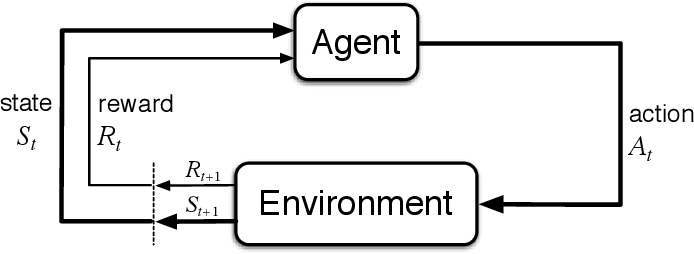
\includegraphics[width=10cm]{figures/1_background_lit_figs/agent_env_interaction.png}
    \caption{Reinforcement learning model (Source: ~\cite{Sutton1998})}
    \label{fig:reinforcement_learning}
\end{figure}

Q-learning~\citep{watkins1992q-learning} is a learning method used for estimating an action-value function,
called the Q value, that forms the basis of modern Reinforcement Learning algorithms. The Q value represents the
estimated discounted reward in the future given an action in a particular state. Equation~\eqref{eq:q_value} gives a
mathematically description where rewards in the future are discounted. A recursive version of this equation can be
formulated as equation~\eqref{eq:q_learning_recursive} where the next state is the max Q value of the next state-action.
Agents can be trained to approximate the Q value using equation~\eqref{eq:q_learning} through the used of a table
of state action pairs.

\begin{align}
    Q(s_t, a_t) = E[R_{t+1} + \gamma R_{t+2} + \gamma^2 R_{t+2} + \cdots ] \label{eq:q_value} \\
    Q(s_t, a_t) = r_t + \gamma \text{max}_a Q(s_{t+1} , a) \label{eq:q_learning_recursive} \\
    Q(s_t, a_t) = Q(s_t, a_t) + \alpha \cdot (r_t + \gamma \cdot \text{max}_a Q(s_{t+1} , a) - Q(s_t, a_t) ) \label{eq:q_learning}
\end{align}

However the curse of dimensionally was found to be a major problem for using Q learning as the number of states
or actions increased, the table grows exponentially in length as well. This made the method impractical for problems
with large state spaces due to both the table size and the required training time for agents.

Therefore function approximators are used to circumvent this problem, typically done using neural networks due to their
ability to approximate any function~\citep{csaji2001approximation} and to be trained using gradient descent.
Work by~\cite{atari}, implemented a deep Q network (DQN) to achieve state-of-the-art performance in six
of seven games tested as part of the Atari game engine, with three of these scores being superhuman. This was done
through using of two different neural network, a model and target network in which the target network is slowly
updated by the model network to act as a slowly updating target Q value. An experience replay buffer was also
implemented to enable the agent to learn from previous actions. \\
Follow up work by~\cite{mnih2015humanlevel} found that with no modifications to the hyperparameters, neural network or
training method; state-of-the-art results were achieved in almost all 49 Atari games with superhuman results in 29 of
these games. The work showed that deep neural networks could be trained through observing just the raw game pixels and
of the game score over time to achieve scores better than those humanly possibly.

Due to this research, a large number of heuristics have been proposed to the loss function~\citep{doubledqn},
network architecture~\citep{duelingdqn}, experience replay buffer~\citep{prioritizedexperiencereplay} and more to
improve the algorithm. A combined agent~\citep{rainbow} applying a range of heuristics enabling it to
achieved over 200\% of the original DQN algorithm in score.

\begin{wrapfigure}{l}{0.5\textwidth}
    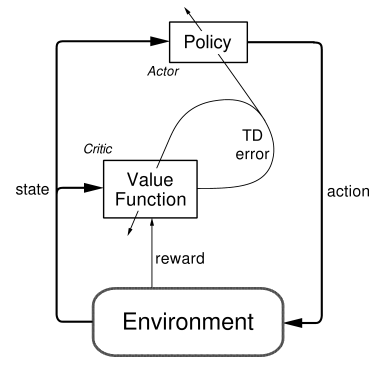
\includegraphics[width=0.5\textwidth]{figures/1_background_lit_figs/actor-critic.png}
    \caption{Actor Critic model (Source: ~\cite{Sutton1998})}
    \label{fig:actor-critic-model}
\end{wrapfigure}

Policy gradient agents, shown in figure~\ref{fig:actor-critic-model}, using the base of Q-learning separate the action
selection policy from the Q-value function known as the critic. In deep Q networks, actions are selected on the maximum
Q-value for all of the actions, however this requires actions to be discretized. By splitting the actions from the Q
values, an actor chooses an action based on the environment state allowing for both discrete and continuous action space
to be utilised. The critic network is trained almost identically to the DQN agent except fro the use of a soft target update.
While the actor network is trained through gradient ascent and the critic evaluation to increase the value. This has the
advantage of the action policy being trained directly compare to DQN agents where used an epsilon greedy action selection
policy however agents can also get stuck in local maxima's. As a result policy gradient has been
used to master the game of Go~\citep{silver2017mastering} and achieve top 1\% in both
Dota 2~\citep{OpenAI_dota} and Starcraft 2~\citep{starcraft2} video games.
%! Suppress = NonBreakingSpace

% Add word count of words
%TC:group table 0 1

\chapter{Optimising Resource Allocation in MEC}
\label{ch:optimising-resource-allocation-in-mec}
In Chapter~\ref{ch:introduction}, the problem that this project aims to address was outlined along with a short
description of the proposed solution. This chapter builds upon that, giving a formal mathematical model for the problem
in Section~\ref{sec:resource-allocation-optimisation-problem}. Section~\ref{sec:auctioning-of-tasks} proposes an
auction mechanism in order to pay servers for their resources in order to deal with self-interested users and as servers
are normally paid for use of their services.

Using the optimisation problem and auction mechanism from the previous sections, agents for both auction and resource
allocation are proposed, in Section~\ref{sec:server-agents}, that learn together to maximise a server's profits
over time.

\section{Resource Allocation Optimisation Problem}
\label{sec:resource-allocation-optimisation-problem}
Using the flexible resource principle, the time taken for a operation to occur, e.g.\ loading of data, computing
a program and sending back results, etc, is proportional to the amount of resources allocated to complete the operation.
A modified version of a resource allocation optimisation model can be designed by building upon the formulation
in~\cite{FlexibleResourceAllocation}.

A sketch of the whole system is in Figure~\ref{fig:system-model}.
The system is assumed to contain a set of $I = \{1,2,\ldots,\left|I\right|\}$ servers that are heterogeneous in all
characteristics. Each server has a fixed resource capacity: storage for the code/data needed to run a task,
measured in GB, computation capacity in terms of CPU cycles per time interval, measured in GHz,
and communication bandwidth to receive the data and to send back the results of the task after execution
measured in Mbit/s. An example of a task could be the analysis of CCTV images with 2GB of data, 5GHz of CPU
cycles and 5MB of results data. The resources for a server $i$ are denoted: $S_i$ for storage capacity, $W_i$ for
computation capacity, and $R_i$ for communication capacity. The system occurs over discrete time steps that are defined
as the set $T = \{1,2,\ldots,\left|T\right|\}$.

\begin{wrapfigure}{l}{0.5\textwidth}
    \centering
    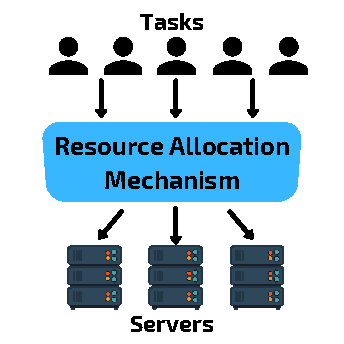
\includegraphics[width=0.5\textwidth]{figures/3_solution_figs/system_model.pdf}
    \caption{System model}
    \label{fig:system-model}
\end{wrapfigure}

The system is assumed to contain a set of $J = \{1,2,\ldots,\left| J \right|\}$ heterogeneous tasks that require
services from one of the servers in set $I$. To run any of these tasks on a server requires storing the appropriate
code/data on the same server. This could be, for example, a set of images, videos or neural network layers used in
identification tasks. \\
The storage size of task $j$ is denoted as $s_j$ with the rate at which the program is transferred to a server at time
$t$ being $s^{'}_{j,t}$. For a task to be computed successfully, it must fetch and execute instructions
on a CPU. We consider the total number of CPU cycles required for the program to be $w_j$, where the number of
CPU cycles assigned to the task at time $t$ is $w^{'}_{j,t}$. Finally, after the task is run and
the results obtained, the latter needs to be sent back to the user. The size of the results for task $j$ is denoted by
$r_j$, and the rate at which they are sent back to the user is $r^{'}_{j,t}$ on a server at time $t$. \\
The allocation of tasks to a server is denoted by $x_{i,j}$ for each task, $j \in J$, and server, $i \in I$. This is
constrained by equation~\eqref{eq:server-task-allocation} meaning that a task can only be allocated to a single server
at any point in time.

\begin{align}
    & \sum_{i \in I} x_{i,j} \leq 1 && \forall{j \in J} \label{eq:server-task-allocation} \\
    & x_{i,j} \in \{0, 1\} && \forall{i \in I, j \in J} \label{eq:server-task-binary}
\end{align}

As the task must complete each stage in series, additional variables are required to track the progress of
each task stage. $\hat{s}_{j,t}$ denotes the loading progress (equation \eqref{eq:loading-progress}), $\hat{w}_{j,t}$
denotes the compute progress (equation~\eqref{eq:compute-progress}) and $\hat{r}_{j,t}$ denotes the sending progress
(equation~\eqref{eq:sending-progress}) of the task. Each of these variables are updated recursively depending
on the progress at the previous time step with the resources allocated. For the compute and sending progress
constraints, the resources allocated are clipped so that the previous stage finishes before the next
stage starts. For each task stage, progress is limited to the total resource required to prevent unneeded resource
allocation (constraints~\eqref{eq:loading-progress-limit},~\eqref{eq:compute-progress-limit}
and~\eqref{eq:sending-progress-limit}).

\begin{align}
    & \hat{s}_{j,t+1} = \hat{s}_{j,t} + s^{'}_{j,t} && \forall{j \in J, t \in T } \label{eq:loading-progress} \\
    & \hat{w}_{j,t+1} = \hat{w}_{j,t} + w^{'}_{j,t} \lfloor{\frac{\hat{s}_{j,t}}{s_j}}\rfloor && \forall{j \in J, t \in T } \label{eq:compute-progress} \\
    & \hat{r}_{j,t+1} = \hat{r}_{j,t} + r^{'}_{j,t} \lfloor{\frac{\hat{w}_{j,t}}{w_j}}\rfloor && \forall{j \in J, t \in T } \label{eq:sending-progress} \\
    & \hat{s}_{j,t} \leq s_j && \forall{j \in J, t \in T} \label{eq:loading-progress-limit} \\
    & \hat{w}_{j,t} \leq w_j && \forall{j \in J, t \in T} \label{eq:compute-progress-limit} \\
    & \hat{r}_{j,t} \leq r_j && \forall{j \in J, t \in T} \label{eq:sending-progress-limit}
\end{align}

Every task has an auction time, denoted by $a_j$ and a deadline, denoted by $d_j$. This is the time step when the task
is auctioned and the last time for which the task can be completed successfully. Using this deadline constraint can be
constructed such that the sending results progress is equal to the required results data at the deadline time step
(equation~\eqref{eq:deadline}).

\begin{align}
    & \hat{r}_{j, d_j} = r_j && \forall{j \in J} \label{eq:deadline}
\end{align}

As servers have limited capacity, the total resource usage for all tasks running on a server must be capped.
The storage constraint (equation~\eqref{eq:server-storage-capacity}) is the sum of the loading progress for
each task allocated to the server. While the computation capacity (equation~\eqref{eq:server-computation-capacity}) is
the sum of compute resources used by all of the tasks on a server $i$ at time $t$ and the bandwidth capacity
(equation~\eqref{eq:server-bandwidth-capacity}) being less than the sum of resources used to load and send results back
by all allocated tasks.

\begin{align}
    & \sum_{j \in J} \hat{s}_{j,t} x_{i,j} \leq S_i && \forall{i \in I, t \in T} \label{eq:server-storage-capacity} \\
    & \sum_{j \in J} w^{'}_{j,t} x_{i,j} \leq W_i && \forall{i \in I, t \in T} \label{eq:server-computation-capacity} \\
    & \sum_{j \in J} (s^{'}_{j,t} + r^{'}_{j,t}) x_{i,j} \leq R_i && \forall{i \in I, t \in T} \label{eq:server-bandwidth-capacity}
\end{align}

\section{Auctioning of Tasks}
\label{sec:auctioning-of-tasks}
While the mathematically description of the problem presented in the previous section doesn't consider any auctions
occurring. In real life servers are normally paid for the use of their resources through auctions as discussed in
Section~\ref{sec:resource-allocation-and-pricing-in-cloud-computing}. However the modifications
that this project has made, all of the auction mechanisms discussed in the previous Chapter are incompatible
due to users not requesting a fixed amount of resources. Nor can the available resources be easily computed as this is
dynamic, depending on the different stages of tasks allocated to a server. The modifications also effect the algorithms
presented in~\cite{FlexibleResourceAllocation} as they assume that all of the task stages can occur concurrently that
this project does not. Because of this, an outline of the most common auctions is presented in
Table~\ref{tab:auctions-descriptions} with their respective properties in Table~\ref{tab:auction-properties} for
selecting an auction mechanism to use.

\begin{longtable}{|p{3.5cm}|p{11cm}|} \hline
    \textbf{Auction type} & \textbf{Description} \\ \hline
    English Auction & A traditional auction where all participants can bid on a single item with the price slowly
        ascending till only a single participant is left who pays the final bid price. Due to the number of rounds,
        this requires a large amount of communication. \\ \hline

    Dutch Auction & The reverse of the English auction, where the starting price is higher than anyone is willing to
        pay with the price slowly dropping till the first participant "jumps in". This can result in sub-optimal pricing
        if the starting price is not high enough or possibly a large number of rounds until anyone bids. Plus due
        the auctions occurring over the internet, latency can have a large effect on the winner. \\ \hline

    Japanese Auction & Similar to the English auction, the Japanese auction is instead over a set period of time lets
        bids increasing with the last bid being the winner. Because of this, there is no guarantee that the price will
        converge to the maximum price like the English but the auction has a fixed time length. However factors like
        latency can have a large effect on the winner and resulting price like the Dutch auction. \\ \hline

    Blind Auction & Also known as a First-price sealed-bid auction, all participants submit a single secret bid for an
        item with the highest bid winning. As a result, no dominant strategy exist as an agent would wish to bid only a
        small amount more than the next highest price in order to not overpay for an item. But due to there being only
        a single round of biding, latency doesn't affect the winner and can occur over a fixed period of time. \\ \hline

    Vickrey Auction~\citep{vickrey} & Also known as a second-price sealed-bid auction, participants each submit
        a single secret bid for an item with the highest bid winning like the blind auction. However the winner only
        pays the price of the second highest bid. Because of this, the dominant strategy (referred to as incentive
        compatibility) for an agent to bid its true value as even if the bid is much higher than all other participants
        its doesn't matter as they pay the minimum required for them to win. \\ \hline
    \caption{Table of Auction mechanisms}
    \label{tab:auctions-descriptions}
\end{longtable}

\begin{table}[h]
    \centering
    \begin{tabular}{|l|c|c|c|} \hline
        \textbf{Auction}  & \textbf{Incentive compatible} & \textbf{Fixed time length} \\ \hline
        English           & False                         & False            \\ \hline
        Dutch             & False                         & False            \\ \hline
        Japanese          & False                         & True             \\ \hline
        Blind             & False                         & True             \\ \hline
        Vickrey           & True                          & True             \\ \hline
    \end{tabular}
    \caption{Table of Auction Properties}
    \label{tab:auction-properties}
\end{table}

The auction properties that this project considers most important are if the fixed time length, which enables fast
auctions for processing large numbers of tasks quickly, and Incentive Compatibility such that an optimal strategy actually exists.
Because of these two properties, the Vickrey Auction~\citep{vickrey} is selected over the alternatives. An additional
advantage of incentive compatibility, is that agents don't need to learn how to outbid another agents, they only need to
learn to accurately evaluate each task allowing agents to learn purely through self-play.

However a modification must be made to the auction as servers generate the prices for tasks rather than the task
suggesting a price to the servers. Because of this, the auction is reversed, such that the bid with the minimum price
wins the task instead of the maximum price. The auction therefore works by allowing all servers to submit their bids for
a task with the winner being the server with the lowest price, but as this is a Vickrey auction, the server actually
gains second lowest price.

\section{Server Agents}
\label{sec:server-agents}
Using the optimisation formulation and auction mechanism from the previous two sections, the problem can be modelled as
Markov Decision Process~\citep{Bel} as shown in Figure~\ref{fig:mdp-system-model}. This has the advantage of separating
out the auction and resource allocation parts of the problem with separate agents acting for each.
Subsection~\ref{subsec:auction-agents} and~\ref{subsec:resource-allocation-agents} proposes agents
for each of the auction and resource allocation environments respectively.

\begin{figure}[H]
    \centering
    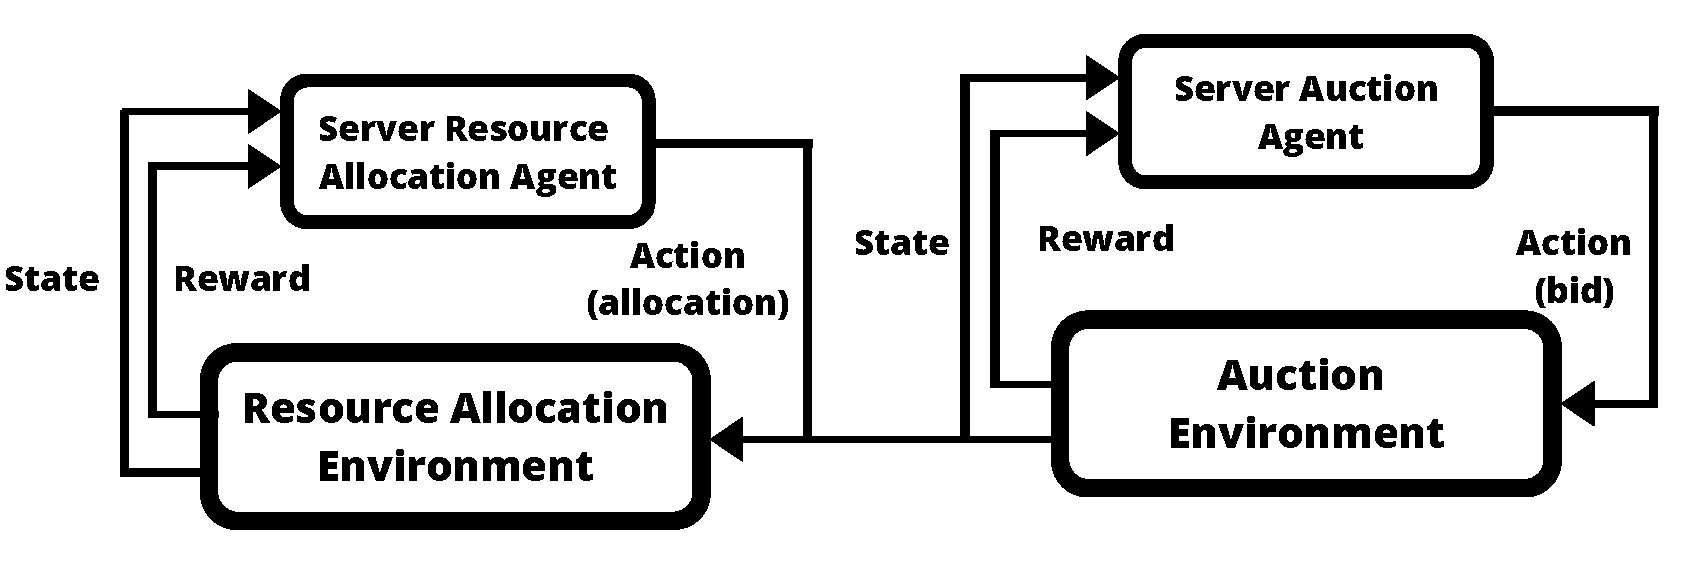
\includegraphics[width=14cm]{figures/3_solution_figs/flexible_resource_allocation_env.pdf}
    \caption{Markov Decision process system model}
    \label{fig:mdp-system-model}
\end{figure}

Due to the exploratory nature of the project, a range of reinforcement learning algorithms and neural network
architectures will be implemented and compared to evaluate the effectiveness of each. These are outlined in
Table~\ref{tab:reinforcement-learning-algorithms} for proposed algorithms and Table~\ref{tab:neural-network-layers} for
networks architectures.

\begin{longtable}{|p{5cm}|p{10cm}|} \hline
    \textbf{Algorithm} & \textbf{Description} \\ \hline
    Dqn~\citep{mnih2015humanlevel} & A standard deep Q network (Dqn) agent that discretizes the action space with a
        target neural network and experience replay buffer. \\ \hline
    Double Dqn~\citep{doubledqn} & A heuristic for the Dqn that modifies the loss function using the target network
        actions index but the model network value. \\ \hline
    Dueling Dqn~\citep{duelingdqn} & A heuristic for the Dqn that modifies the network to separates the state value
        and action advantages that can help understand the environment. \\ \hline
    Categorical Dqn~\citep{distributional_dqn} & DQN represents the Q value as a scalar value, the Categorical DQN agent
        outputs probability distribution over values which is helpful for environments that are stochastic. \\ \hline
    Deep Deterministic Policy Gradient~\citep{ddpg} & Deep Deterministic Policy Gradient (DDPG) allows for continuous
        actions space, compared to DQN agents that must discretize the action space. This is done through the use of an
        actor and critic network with target networks for each that are updated with a soft target update method. \\ \hline
    Twin Delay DDPG~\citep{td3} & Like the Double Dueling DQN agents, Twin delay DDPG (TD3) includes a couple
        heuristics for the DDPG algorithm. A critic twin is used to prevent the actor network from tricking the critic
        network in evaluating a state's Q value. Another heuristic is the delaying the updates for actor network
        compared to the critic network to allow the critic to out learn the actor to prevent being tricked.\\ \hline
    Td3 Central critic & As there are multiple agents working together, the critic used for all of the agents can be
        same, this is inspired by~\cite{maddpg} which the critic only evaluates the agents private observation not with
        complete information of all agents. \\ \hline
    \caption{Table of the Reinforcement Learning algorithms}
    \label{tab:reinforcement-learning-algorithms}
\end{longtable}

\begin{longtable}{|p{3.5cm}|p{12cm}|} \hline
    \textbf{Neural Network} & \textbf{Description} \\ \hline
    Artificial Neural Networks \citep{ANN} & Originally developed as a theoretically approximation for the brain, it
        was found that for networks with at least one hidden layer, networks could approximate any
        function~\citep{csaji2001approximation}. This made neural networks extremely helpful for cases where it would
        normally be too difficult for a human to specify the exact function, neural networks can be used to find a
        close approximation to the true function through gradient descent. \\ \hline

    Recurrent Neural Network~\citep{RNN} & A major weakness of artificial neural networks is in its use of a fixed
        number of inputs and outputs making them unusable with text, sound or video where previous inputs are important
        for understanding a current input. Therefore recurrent neural network's (RNN) extend artificial neural networks
        to allow for connections to previous neurons to "pass on" information. However this was found to struggle from
        vanishing or exploding gradient during training such that gradients would tended either to zero or infinity
        over long sequences. \\ \hline

    Long/Short Term Memory \citep{LSTM} & Long/Short Term memory (LSTM) aims to remedy RNNs problem of vanishing and
        exploding gradient problems. This is done by using forget gates that determine how much information from the
        last state would get, allowing for more complex information to be remembered over time compared to RNNs. \\ \hline

    Gated Recurrent unit~\citep{GRU} & Gated recurrent unit (GRU) are very similar to LSTMs, except for the use of
        different wiring mechanisms with one less gate, an update gate instead of two forget gates. These changes mean
        that GRUs run faster and are easier to code than LSTMs. However are not as expressive meaning that less complex
        functions can be encoded. \\ \hline

    Bidirectional \citep{Bidirectional} & With RNNs, LSTMs and GRUs, inputs are passed through forward however in
        understanding an input the subsequent inputs are also required. Bidirectional neural network fixed this by
        passes in an input twice, once forwards normally and then a second time in reverse. This allows networks to
        understand the context around an input from both before it and after it. \\ \hline

    Neural Turing Machine~\citep{NTM} & Inspired by computers, Neural Turing Machines build on long/short term memory
        by using an external memory module instead of memory being inbuilt to the network. This allows for external
        observers to understand what is going on much better than other networks due to their black-box nature. \\ \hline

    Differentiable Neural Computer~\citep{DNC} & An expansion to the Neural Turing Machine that allows the memory
        module to be scalable in size allowing for additional memory to be added if needed. \\ \hline

    Sequence to Sequence Network \citep{seq2seq} & All networks considered above allow for sequences to be passed in
        while outputting a single output vector. Sequence to sequence (Seq2Seq) networks utilise two sub-networks; an
        encoder and decoder. The encoder takes a sequence that is encoded which is outputted to the decoder that then
        outputs another sequence by continually passing in the decoders last input. \\ \hline
    \caption{Table of Neural network layers}
    \label{tab:neural-network-layers}
\end{longtable}

\subsection{Auction Agents}
\label{subsec:auction-agents}
Traditionally pricing mechanisms~\citep{al2013cloud} rely on mixture of metrics: resource availability, resource demand,
quality of service, task resource allocation quantity, etc to determine a price. However
these values are difficult to approximate during the auction for this project. So, due to the complexity of
deriving this function, reinforcement learning will be used to learn an optimal policy for a server to maximise its
profits over time.

\begin{figure}[H]
    \centering
    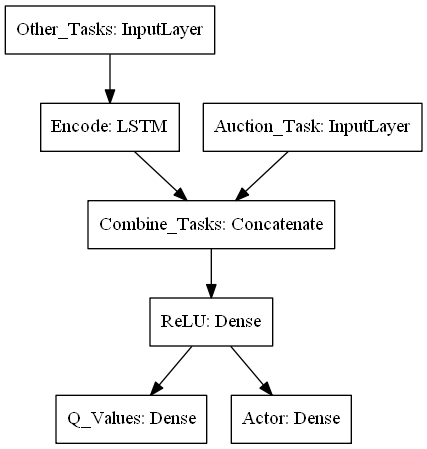
\includegraphics[width=0.5\textwidth]{figures/3_solution_figs/task_pricing_network_architecture.png}
    \caption{Task pricing network architecture}
    \label{fig:task-pricing-network-architecture}
\end{figure}

The network used for the auction must take into account a server's current tasks and the attributes of the task being
auctioned. Because of this, a recurrent network must be used like the RNN, GRU, LSTM and Bidirectional as the number
of tasks allocated to a server is unknown. For the DDPG, a single ReLU output will be used while a linear Q value output
for DQN agent must be used as shown in Figure~\ref{fig:task-pricing-network-architecture}.

\subsection{Resource Allocation Agents}
\label{subsec:resource-allocation-agents}
When a new task is allocated to the server or a task completes a stage, the server will need to redistributed its
resources to its tasks. But while the problem of how to allocate resources isn't as complex as the task pricing policy
in Section~\ref{subsec:auction-agents}, no obvious heuristics exist. This is because allocation of resources to a single
task must take into account other tasks that it will affect in order to balance resources between allocated tasks.
Because of this, reinforcement learning agents are proposed to learn this with two
different network structures and a weighting heuristic to simplify the optimal function for agents.

The heuristic proposes that a weighted value for the task's resources is used instead of the raw resource usage of a
task. While simpler, this approach still has the same expressiveness as the exact resource usage while avoiding
the problem of either over or under allocating resources to tasks.

\begin{figure}[H]
    \centering
    \begin{minipage}{0.45\linewidth}
        \centering
        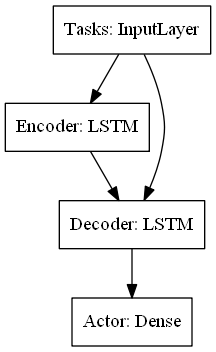
\includegraphics[width=\linewidth]{figures/3_solution_figs/multi_task_actor_weighting_network_architecture.png}
        \caption{Multi-task Seq2Seq actor network architecture}
        \label{fig:seq2seq-actor-network-architecture}
    \end{minipage}\hfill
    \begin{minipage}{0.55\linewidth}
        \centering
        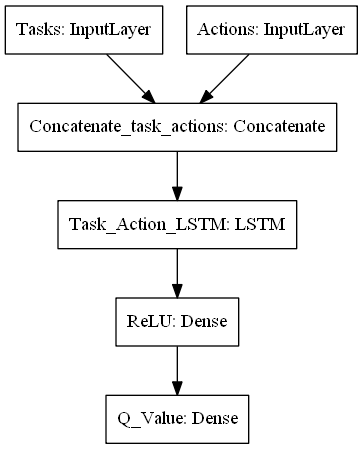
\includegraphics[width=\linewidth]{figures/3_solution_figs/single_task_critic_weighting_network_architecture.png}
        \caption{Multi-task Seq2Seq critic network architecture}
        \label{fig:seq2seq-critic-network-architecture}
    \end{minipage}
\end{figure}

To allocate resources to a single task requires also being aware of the resource requirements of other tasks. Because
of this, two different neural network structures are proposed, one using a Sequence to Sequence network to allow
all tasks actions to be determined simultaneously and the other structure weights a single task at a time. For the
Sequence to Sequence network, all tasks are passed in to the encoder that allows the task's attributes to be compressed
before passing its output the decoder as shown in Figure~\ref{fig:seq2seq-actor-network-architecture}. However Dqn can't
be used to train the network therefore a critic network, Figure~\ref{fig:seq2seq-critic-network-architecture}, is
required for policy gradient training. \\
The alternative network uses a simple recurrent neural networks but due to having to output a fixed shape, only a
single task can be weighted at a time, as shown in Figure~\ref{fig:resource-weighting-network-architecture}. Because of
this, each task is required to pass through the network. However this network structure can be trained with both
Dqn and policy gradient algorithms unlike the Sequence to Sequence network. The Neural Machine Machine and
Differentiable Neural Computer were not implemented due to there complexity.

\begin{figure}[h]
    \centering
    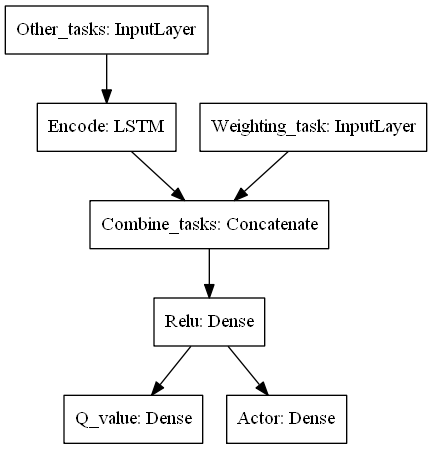
\includegraphics[width=0.75\textwidth]{figures/3_solution_figs/single_task_weighting_network_architecture.png}
    \caption{Single task resource weighting network architecture}
    \label{fig:resource-weighting-network-architecture}
\end{figure}



\chapter{Implementation of the solution}\label{ch:implementation-of-the-solution}

% Texcount ignores the longtables
%TC:group table 0 1

\chapter{Testing and evaluation}\label{ch:testing-and-evaluation}
Using the implemented solution from Chapter~\ref{ch:implementation-of-the-solution} to test and evaluate its
effectiveness, both functional unit tests and agent training evaluation have been designed. To confirm that the
environment and agents implemented in the previous chapter
(section~\ref{sec:implementing-auction-and-resource-allocation-agents}) works as intended, unit testing has been added
that is explained in Section~\ref{sec:functional-testing}. While to evaluate the effectiveness of the proposed
solution from Section~\ref{sec:proposed-agents}, a range of metric have been measured during training in order to
test and compare implemented agents, neural network architectures and training parameters. These results are explained
in Section~\ref{sec:agent-evaluation}.

\section{Functional testing}\label{sec:functional-testing}
To confirm that the implementation of the agents and environment correctly, PyTest a module within Python has been used
to design functions are valid. These tests are split into three families: agent, environment and training that are
explained in the respective tables~\ref{tab:agent_testing},~\ref{tab:env_testing} and~\ref{tab:training_testing}.
The results from the testing is shown in figure~\ref{fig:pytest_results}.

\begin{longtable}{|p{3cm}|p{11cm}|} \hline
    \textbf{Test name} & \textbf{Explanation} \\ \hline
    Building agents & Constructs all of the agents with possible arguments to confirm agents can accept of all its
        attributes\\ \hline
    Saving agents & Confirms that agents can successfully save their neural networks and can successfully load
        the network again and is equal to the agent network. \\ \hline
    Agent actions & Confirms that all agents can generate valid actions for both bidding and weighting \\ \hline
    Gin config file & Gin is used to set the arguments used during training, to confirm that the file is valid. \\ \hline
    Building networks & Constructs all of the neural networks to confirm that the network return a valid output. \\ \hline
    Agent epsilon policy & While training, some of the agent actions are randomly selected to train the agents over
        a large area of the state. This tests that the random actions selected are valid. \\ \hline
    \caption{Table of test functions of the agents}
    \label{tab:agent_testing}
\end{longtable}

\begin{longtable}{|p{3cm}|p{11cm}|} \hline
    \textbf{Testing name} & \textbf{Explanation} \\ \hline
    Saving and loading an environment & The environment allows for the saving the environment at its current
        state. This tests that the environment can save and reload the environment successfully. \\ \hline
    Loading environment settings & Tests that the load environment settings correctly generates a new random
        environment based on the settings. \\ \hline
    Random action environment steps & Tests that inputs to the auction and resource allocation steps work,
        random actions are generated to check for environment edge cases.  \\ \hline
    Auction step & To confirm the Vickrey auction mechanism is completely implemented, a range of possible inputs
        are tested to confirm that right price and server that the task is allocated. \\ \hline
    Resource allocation step & To confirm that servers allocate their resources correct given some inputs. \\ \hline
    Allocation of computational resources & Checks that the server correctly allocates computational resources to
        allocated tasks. \\ \hline
    Allocation of storage and bandwidth resources & Checks that the server correctly allocates storage and
        bandwidth resources to allocated tasks. \\ \hline
    Allocation of all resources & Checks that resources are allocated by the server correctly for all of the
        resources. \\ \hline
    \caption{Table of test functions of the environment}
    \label{tab:env_testing}
\end{longtable}

\begin{longtable}{|p{3cm}|p{11cm}|} \hline
    \textbf{Testing name} & \textbf{Explanation} \\ \hline
    Task pricing training & Tests that the task pricing reinforcement learning agents can correctly learning from
        different auction observations. \\ \hline
    Resource allocation training & Tests that resource allocation reinforcement learning agents can correctly
        learn from different resource allocation observations. \\ \hline
    Agent evaluation & Tests that the agent evaluation function during training correctly captures the correct
        information due to the actions taken. \\ \hline
    Agent training & Tests that agents can be correctly trained over an environment with different actions and
        observations. \\ \hline
    Random actions training & Tests that agents with random actions can quickly using the environment training
        methods to confirm that the function work as intended. \\ \hline
    \caption{Table of test functions of agent training}
    \label{tab:training_testing}
\end{longtable}

\begin{figure}[H]
    \centering
    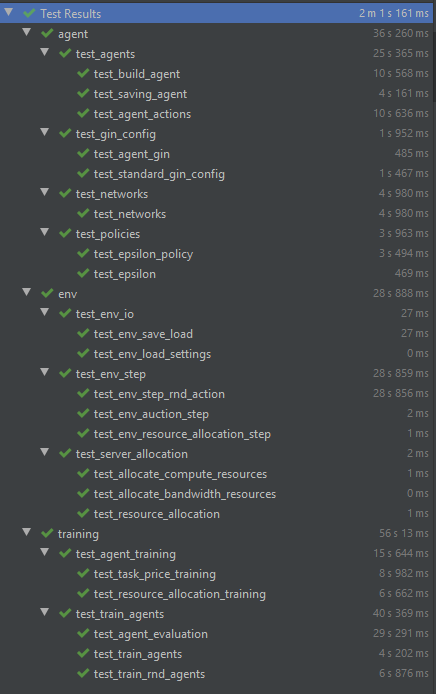
\includegraphics{figures/4_test_eval_figs/pytest_results.PNG}
    \caption{Results of the unit functions described in the Tables~\ref{tab:agent_testing},~\ref{tab:env_testing}
        and~\ref{tab:training_testing}}
    \label{fig:pytest_results}
\end{figure}

\section{Agent evaluation}\label{sec:agent-evaluation}
In order to compare the implemented agents from Chapter~\ref{ch:implementation-of-the-solution}, a range of metric are
used which are recorded while the agent is training. For the auction agent the metrics are: histogram winning prices,
number of no bids, number of failed tasks, number of completed tasks and a histogram of actions taken. For the resource
allocation agents the metrics are a histogram of weighting, number of failed tasks and number of completed tasks.
Using these metrics evaluation of agent performance can be done between the different reinforcement learning algorithms
implemented in Table~\ref{tab:reinforcement_learning_algorithms}, network architectures in
Table~\ref{tab:neural_network_layers} and methods of training different agents. \\
These evaluations fall into three families: env and agent num, algorithm and network architecture that are analysed in
Subsections~\ref{subsec:environment-and-agent-number-training},~\ref{subsec:reinforcement-learning-algorithm-training}
and~\ref{subsec:neural-network-architecture-training} respectively.

\subsection{Environment and Agent number training}\label{subsec:environment-and-agent-number-training}
The analysis of the different reinforcement learning algorithms and neural network architectures in
Subsection~\ref{subsec:reinforcement-learning-algorithm-training} and~\ref{subsec:neural-network-architecture-training}
respectively assume two qualities that this subsection analyses. These are the training and evaluation environments
and the number of agents used during training. As there are huge ranges of possible environment settings that agents
could be trained, investigating agent environment generality is a challenge and an important measure within machine
learning. This is of particular importance for this work, as in real-life, the environment that agents experiences will
can be unpredictable and different from those trained on. Meaning that agents should learn to generalise and not
overfit to particular environments used during training.

The other assume quality is due an advantage of the Vickrey auction over alternative auctions, explored in
Section~\ref{sec:auctioning-of-tasks}, that it is Incentive compatible. This auction property means that the dominant
strategy for all agents is to bid truthfully, which is the agent's true evaluation of the task. Therefore due to agents
not needing to learn to "out bid" each other allowing for effective self-play to be used in training.

Therefore this subsection compare the results of agents that are trained on a single environment setting and those
trained on multiple environment settings and when multiple or single agents are trained together.
These are compared using a set of pre-generated environments, one from the single environment setting and another from
the multiple environment settings.

%% Env training legend
\begin{wrapfigure}{r}{0.5\textwidth}
    \includegraphics[width=0.5\textwidth]{figures/4_test_eval_figs/env_training_fig/legend.png}
    \caption{Environment training legend}
    \label{fig:env-training-legend}
\end{wrapfigure}

During train, every 10 episodes, the agents are trained on the environments pre-generated from the multi-env settings.
Then in each of these evaluations, five metrics are collected: the number of completed tasks
(figure~\ref{fig:env_num_completed_tasks}), number of failed tasks (figure~\ref{fig:env_num_failed_tasks}),
the percentage of tasks attempted (figure~\ref{fig:env_percent_tasks}), total prices (figure~\ref{fig:env_total_prices})
and total winning prices (figure~\ref{fig:env_winning_prices}) when the environment are run. \\

%% Training evaluation
\begin{figure}[H]
    \centering
    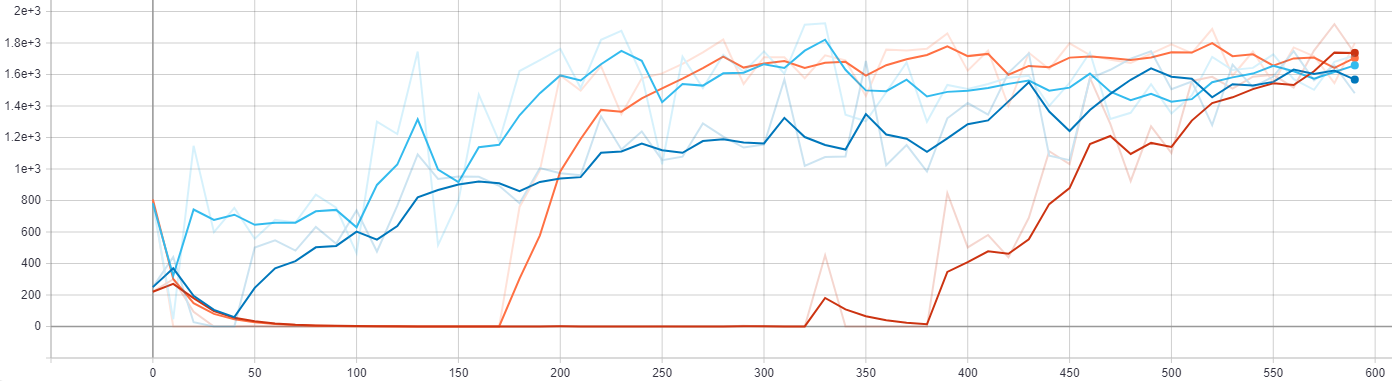
\includegraphics[width=17cm]{figures/4_test_eval_figs/env_training_fig/num_completed_tasks.png}
    \caption{Number of completed tasks}
    \label{fig:env_num_completed_tasks}
\end{figure}

\begin{figure}[H]
    \centering
    \includegraphics[width=17cm]{figures/4_test_eval_figs/env_training_fig/num_failed_tasks.png}
    \caption{Number of failed tasks}
    \label{fig:env_num_failed_tasks}
\end{figure}

\begin{figure}[H]
    \centering
    \includegraphics[width=17cm]{figures/4_test_eval_figs/env_training_fig/percent_tasks.png}
    \caption{Percentage of tasks attempted}
    \label{fig:env_percent_tasks}
\end{figure}

\begin{figure}[H]
    \centering
    \includegraphics[width=17cm]{figures/4_test_eval_figs/env_training_fig/total_prices.png}
    \caption{Total prices}
    \label{fig:env_total_prices}
\end{figure}

\begin{figure}[H]
    \centering
    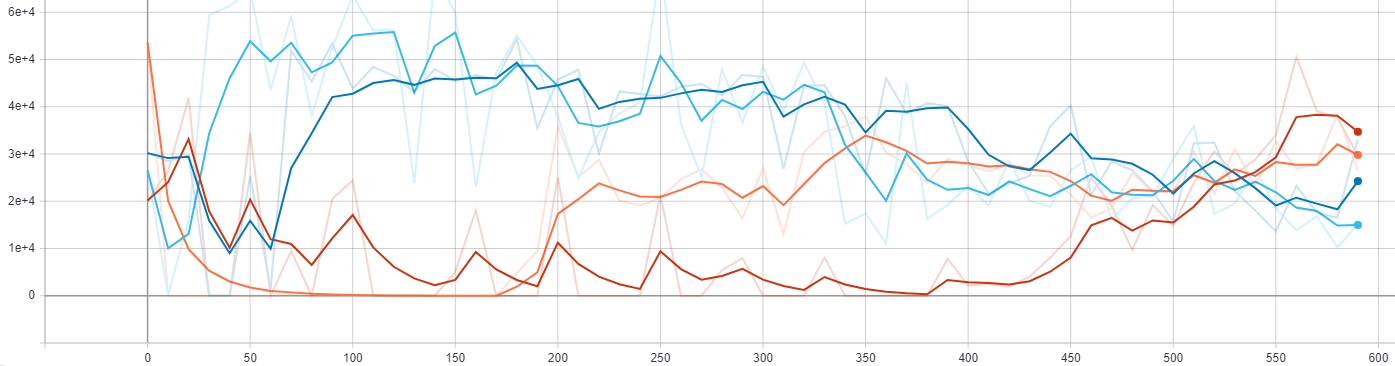
\includegraphics[width=17cm]{figures/4_test_eval_figs/env_training_fig/total_winning_prices.PNG}
    \caption{Total winning prices}
    \label{fig:env_winning_prices}
\end{figure}

%% Analysis of the training results
%% TODO

%% Auction prices and resource weightings histograms
%% TODO but Im not sure this is interesting or needed

\subsection{Reinforcement learning algorithm training}\label{subsec:reinforcement-learning-algorithm-training}
In table~\ref{tab:reinforcement_learning_algorithms}, a range of reinforcement learning algorithms were proposed as
methods of training neural networks. Using the analysis from the previous subsections, during training agents were
trained on multiple environment settings with multiple task pricing agents and a single resource weighting agents.
The evaluation environment were pre-generated as well to confirm uniform testing between the agents. \newline

\begin{wrapfigure}{l}{0.5\textwidth}
    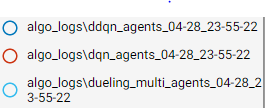
\includegraphics[width=0.5\textwidth]{figures/4_test_eval_figs/algo_training_fig/legend.PNG}
    \caption{Environment training legend}
    \label{fig:algo-training-legend}
\end{wrapfigure}

%% Training evaluation
\begin{figure}[H]
    \centering
    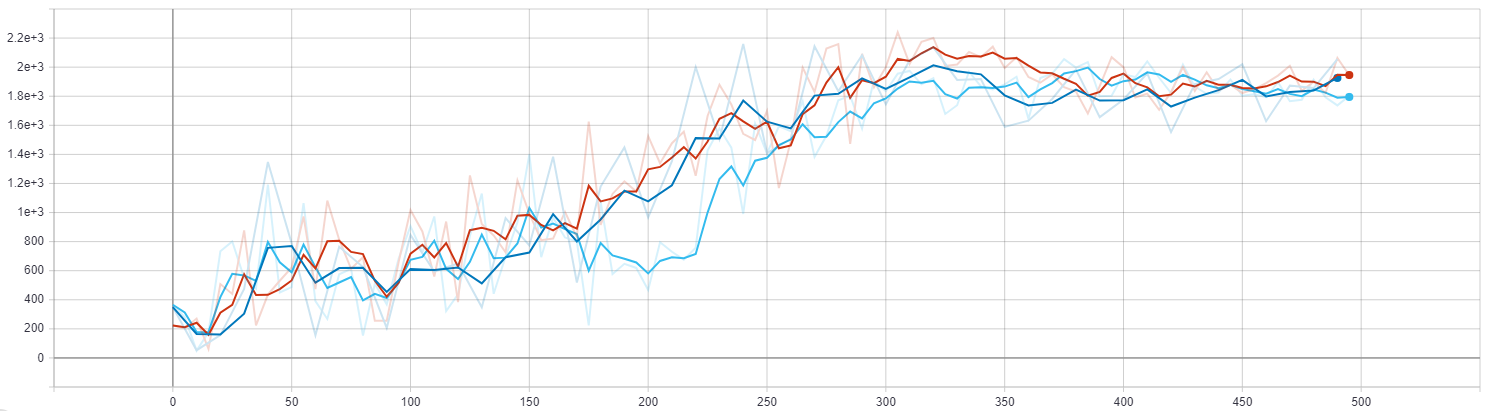
\includegraphics[width=17cm]{figures/4_test_eval_figs/algo_training_fig/num_completed_tasks.PNG}
    \caption{Number of completed tasks}
    \label{fig:algo_num_completed_tasks}
\end{figure}

\begin{figure}[H]
    \centering
    \includegraphics[width=17cm]{figures/4_test_eval_figs/algo_training_fig/num_failed_tasks.png}
    \caption{Number of failed tasks}
    \label{fig:algo_num_failed_tasks}
\end{figure}

\begin{figure}[H]
    \centering
    \includegraphics[width=17cm]{figures/4_test_eval_figs/algo_training_fig/percent_tasks.png}
    \caption{Percent of tasks attempted}
    \label{fig:algo_percent_tasks}
\end{figure}

\begin{figure}[H]
    \centering
    \includegraphics[width=17cm]{figures/4_test_eval_figs/algo_training_fig/total_prices.png}
    \caption{Total prices}
    \label{fig:algo_total_prices}
\end{figure}

\begin{figure}[H]
    \centering
    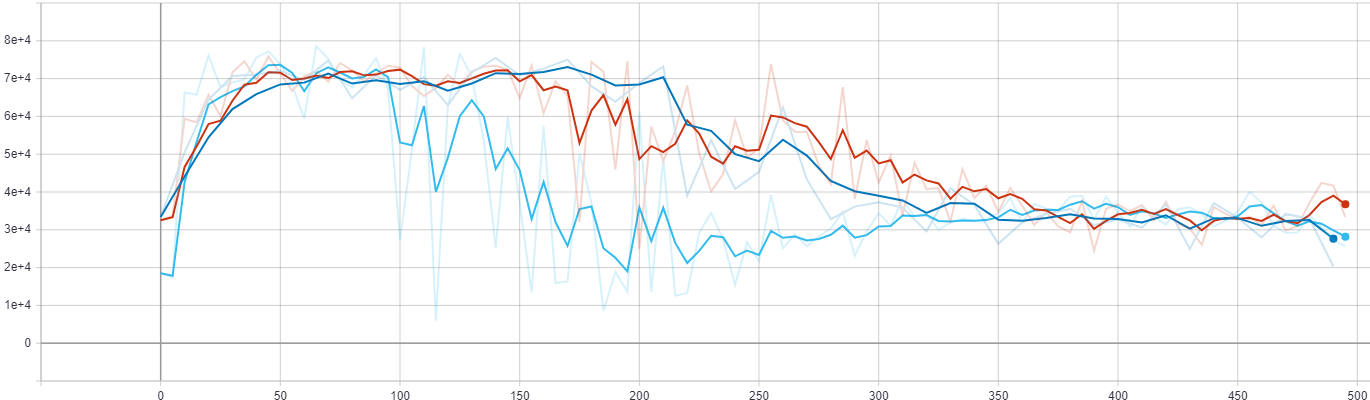
\includegraphics[width=17cm]{figures/4_test_eval_figs/algo_training_fig/total_winning_prices.PNG}
    \caption{Winning prices}
    \label{fig:algo_winning_prices}
\end{figure}

With the agents, an action histogram is recorded for all of the actions taken every 100 episodes to analyse the change
of actions taken over time and to investigate the difference is how algorithms evaluate the value of a position. Each
agent has the the auction and weighting actions separated due to their difference in policy. \newline

\begin{figure}[H]
    \centering
    \begin{minipage}{0.5\textwidth}
        \centering
        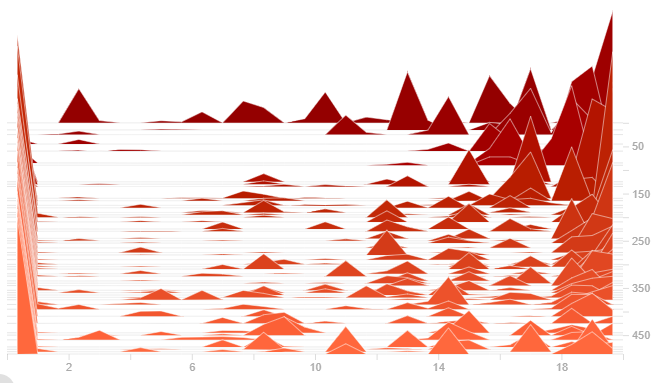
\includegraphics[width=1.0\textwidth]{figures/4_test_eval_figs/algo_training_fig/dqn_auction_prices.png}
        \caption{Deep Q Network auction prices}
        \label{fig:dqn-auction-prices}
    \end{minipage}\hfill
    \begin{minipage}{0.5\textwidth}
        \centering
        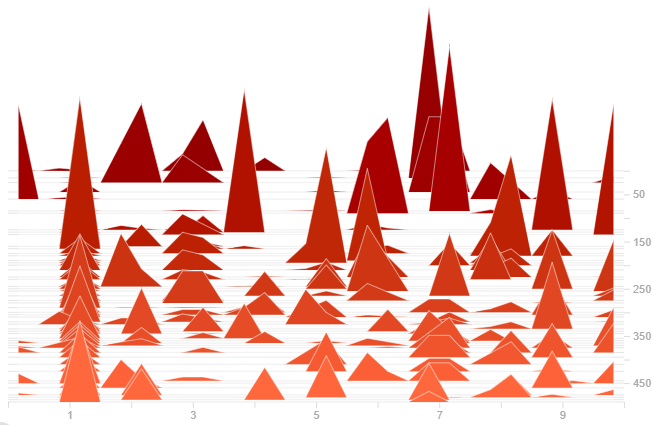
\includegraphics[width=1.0\textwidth]{figures/4_test_eval_figs/algo_training_fig/dqn_weightings.png}
        \caption{Deep Q Network resource weightings}
        \label{fig:dqn-resource-weightings}
    \end{minipage}
\end{figure}

\begin{figure}[H]
    \centering
    \begin{minipage}{0.5\textwidth}
        \centering
        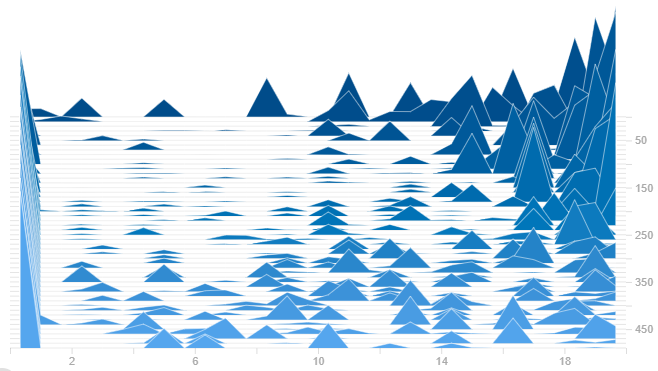
\includegraphics[width=1.0\textwidth]{figures/4_test_eval_figs/algo_training_fig/ddqn_auction_prices.png}
        \caption{Double Deep Q Network auction prices}
        \label{fig:ddqn-auction-prices}
    \end{minipage}\hfill
    \begin{minipage}{0.5\textwidth}
        \centering
        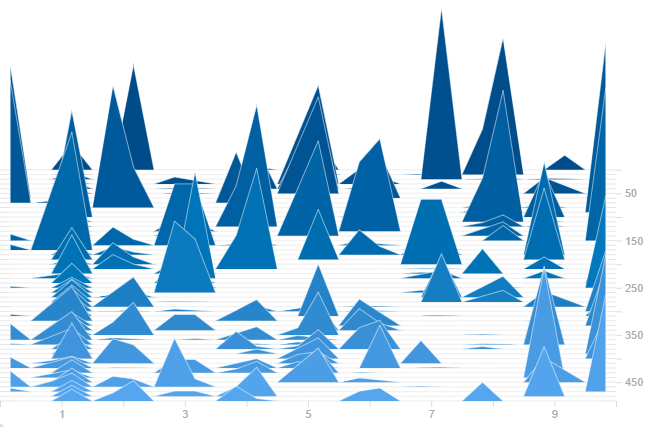
\includegraphics[width=1.0\textwidth]{figures/4_test_eval_figs/algo_training_fig/ddqn_weightings.png}
        \caption{Double Deep Q Network resource weightings}
        \label{fig:ddqn-resource-weightings}
    \end{minipage}
\end{figure}

\begin{figure}[H]
    \centering
    \begin{minipage}{0.5\textwidth}
        \centering
        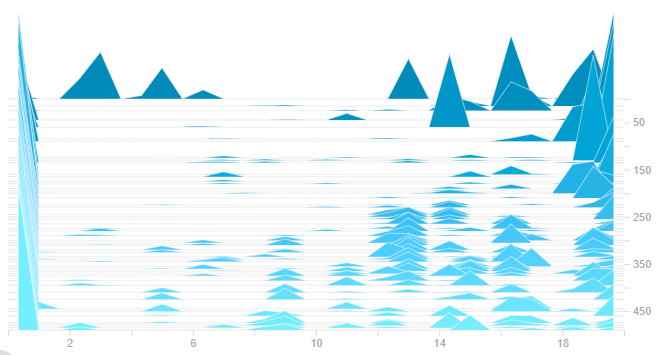
\includegraphics[width=1.0\textwidth]{figures/4_test_eval_figs/algo_training_fig/dueling_dqn_auction_prices.png}
        \caption{Dueling Deep Q Network auction prices}
        \label{fig:dueling-dqn-auction-prices}
    \end{minipage}\hfill
    \begin{minipage}{0.5\textwidth}
        \centering
        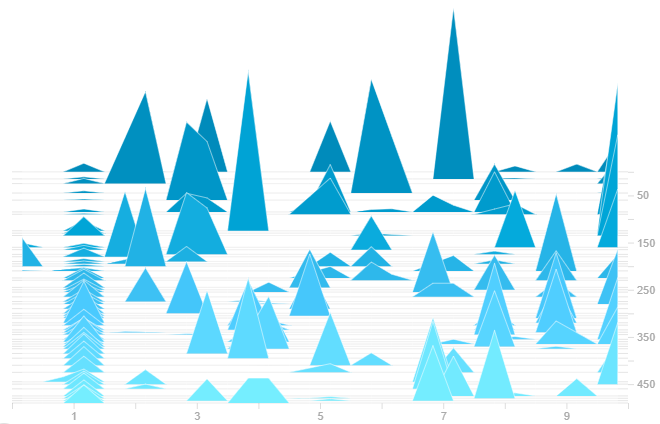
\includegraphics[width=1.0\textwidth]{figures/4_test_eval_figs/algo_training_fig/dueling_dqn_weightings.png}
        \caption{Dueling Deep Q Network resource weightings}
        \label{fig:dueling-dqn-resource-weightings}
    \end{minipage}
\end{figure}

\subsection{Neural network architecture training}\label{subsec:neural-network-architecture-training}
There are a wide-range of compatible neural network architectures that agents can use, as outlined in
table~\ref{tab:neural_network_layers}. To compare these architectures, the DQN agents from the previous subsection is
used due to its effectiveness and simplicity with four different network architectures: RNN~\citep{RNN},
LSTM~\citep{LSTM}, GRU~\citep{GRU} and Bidirectional~\citep{Bidirectional} using an LSTM network. \\

\begin{wrapfigure}{l}{0.5\textwidth}
    \includegraphics[width=0.5\textwidth]{figures/4_test_eval_figs/net_arch_training_fig/legend.png}
    \caption{Environment training legend}
    \label{fig:net-arch-training-legend}
\end{wrapfigure}

%% Training evaluation
\begin{figure}[H]
    \centering
    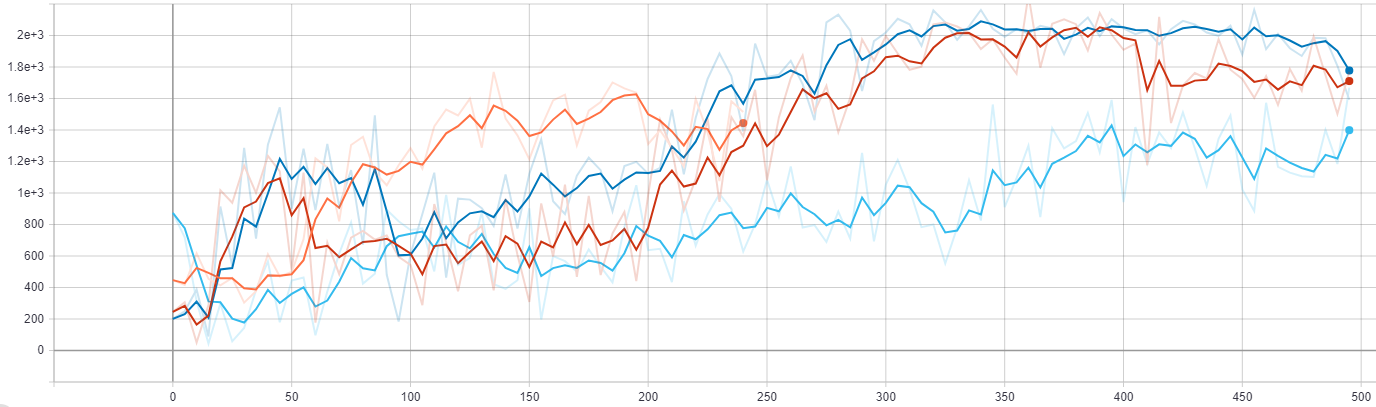
\includegraphics[width=17cm]{figures/4_test_eval_figs/net_arch_training_fig/num_completed_tasks.PNG}
    \caption{Number of completed tasks}
    \label{fig:net_arch_num_completed_tasks}
\end{figure}

\begin{figure}[H]
    \centering
    \includegraphics[width=17cm]{figures/4_test_eval_figs/net_arch_training_fig/num_failed_tasks.png}
    \caption{Number of failed tasks}
    \label{fig:net_arch_num_failed_tasks}
\end{figure}

\begin{figure}[H]
    \centering
    \includegraphics[width=17cm]{figures/4_test_eval_figs/net_arch_training_fig/percent_tasks.png}
    \caption{Percent of tasks attempted}
    \label{fig:net_arch_percent_tasks}
\end{figure}

\begin{figure}[H]
    \centering
    \includegraphics[width=17cm]{figures/4_test_eval_figs/net_arch_training_fig/total_prices.png}
    \caption{Total prices}
    \label{fig:net_arch_total_prices}
\end{figure}

%% TODO may not be needed
\begin{figure}[H]
    \centering
    \begin{minipage}{0.5\textwidth}
        \centering
        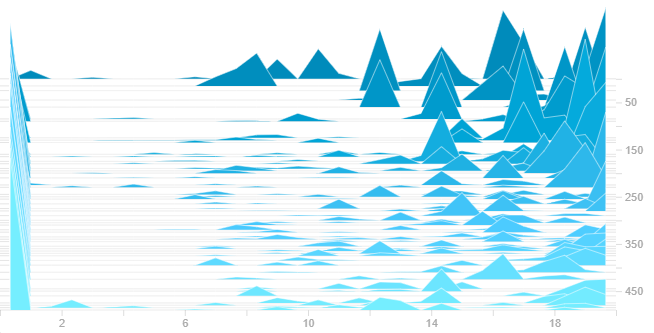
\includegraphics[width=1.0\textwidth]{figures/4_test_eval_figs/net_arch_training_fig/rnn_architecture_auction_prices.png}
        \caption{Rnn network architecture auction prices}
        \label{fig:rnn-auction-prices}
    \end{minipage}\hfill
    \begin{minipage}{0.5\textwidth}
        \centering
        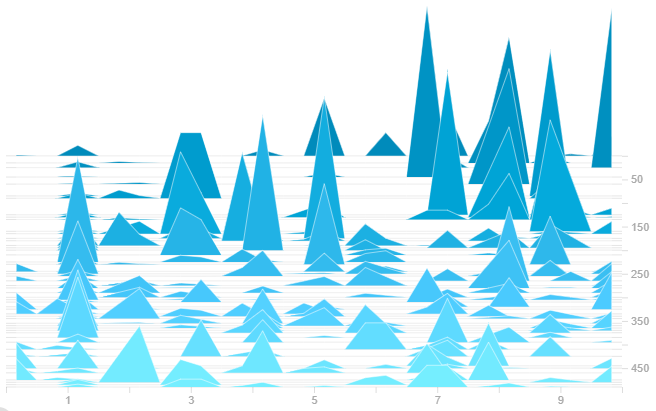
\includegraphics[width=1.0\textwidth]{figures/4_test_eval_figs/net_arch_training_fig/rnn_architecture_weightings.png}
        \caption{Rnn network architecture resource weightings}
        \label{fig:rnn-resource-weightings}
    \end{minipage}
\end{figure}

\begin{figure}[H]
    \centering
    \begin{minipage}{0.5\textwidth}
        \centering
        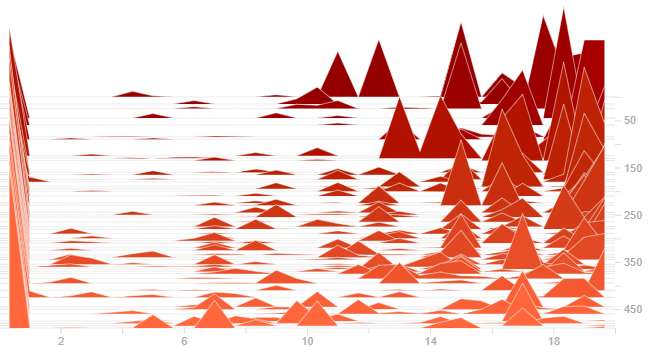
\includegraphics[width=1.0\textwidth]{figures/4_test_eval_figs/net_arch_training_fig/gru_architecture_auction_prices.png}
        \caption{GRU network architecture auction prices}
        \label{fig:gru-auction-prices}
    \end{minipage}\hfill
    \begin{minipage}{0.5\textwidth}
        \centering
        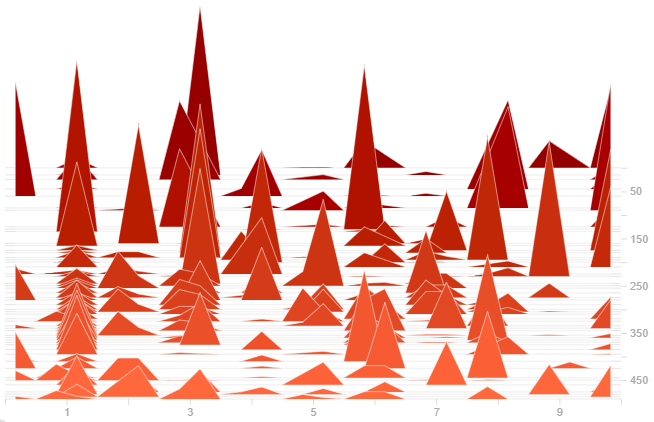
\includegraphics[width=1.0\textwidth]{figures/4_test_eval_figs/net_arch_training_fig/gru_architecture_weightings.png}
        \caption{GRU network architecture resource weightings}
        \label{fig:gru-resource-weightings}
    \end{minipage}
\end{figure}

\begin{figure}[H]
    \centering
    \begin{minipage}{0.5\textwidth}
        \centering
        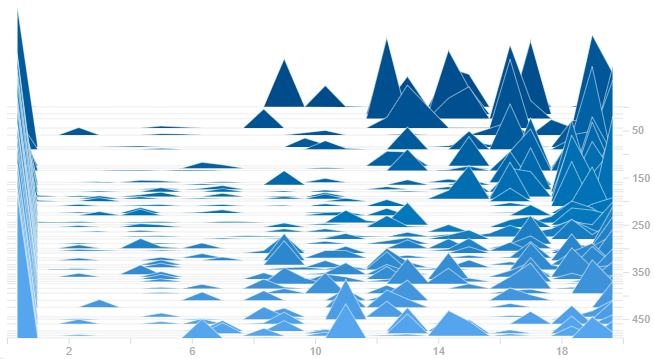
\includegraphics[width=1.0\textwidth]{figures/4_test_eval_figs/net_arch_training_fig/lstm_architecture_auction_prices.png}
        \caption{LSTM network architecture auction prices}
        \label{fig:lstm-auction-prices}
    \end{minipage}\hfill
    \begin{minipage}{0.5\textwidth}
        \centering
        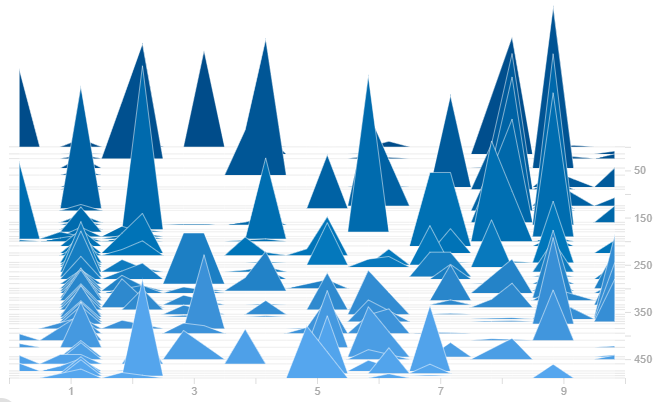
\includegraphics[width=1.0\textwidth]{figures/4_test_eval_figs/net_arch_training_fig/lstm_architecture_weightings.png}
        \caption{Rnn network architecture resource weightings}
        \label{fig:lstm-resource-weightings}
    \end{minipage}
\end{figure}

\begin{figure}[H]
    \centering
    \begin{minipage}{0.5\textwidth}
        \centering
        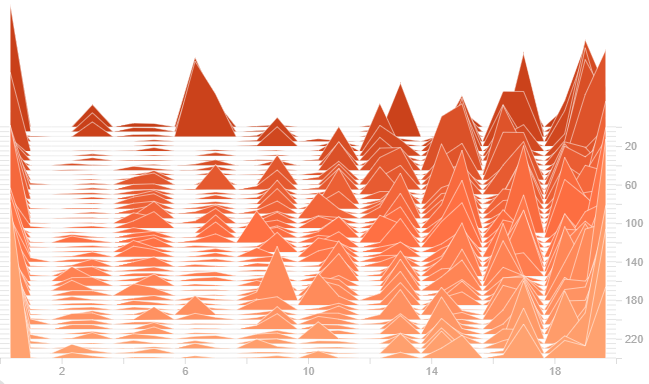
\includegraphics[width=1.0\textwidth]{figures/4_test_eval_figs/net_arch_training_fig/bidirectional_architecture_auction_prices.png}
        \caption{Bidirectional network architecture auction prices}
        \label{fig:bidirectional-auction-prices}
    \end{minipage}\hfill
    \begin{minipage}{0.5\textwidth}
        \centering
        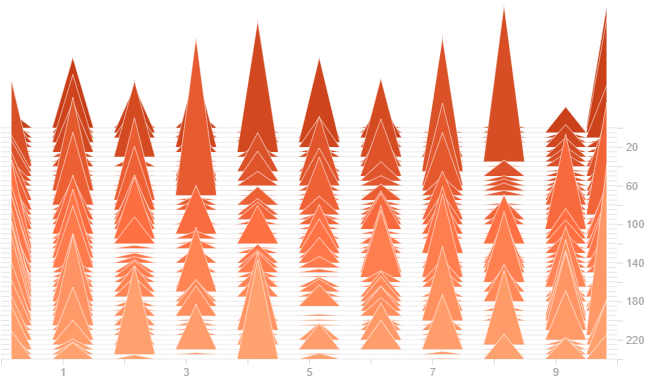
\includegraphics[width=1.0\textwidth]{figures/4_test_eval_figs/net_arch_training_fig/bidirectional_architecture_weightings.png}
        \caption{Bidirectional network architecture resource weightings}
        \label{fig:bidirectional-resource-weightings}
    \end{minipage}
\end{figure}
\chapter{Conclusion and future work}
\label{ch:conclusion-and-future-work}
The aim of this project was to expand previous research to fix flaws in the Flexible resource allocation optimisation
problems for Mobile Edge Computing. This was achieved by introducing the notion of time into the optimisation
model. As a result, a new optimisation problem was presented in Section~\ref{sec:resource-allocation-optimisation-problem}
along with an auction mechanism to deal with self-interested users (Section~\ref{sec:auctioning-of-tasks}). \\
Due to the complexity of the problem, Reinforcement learning was applied to learn how to bid on auctioned tasks and
allocation the server's resources. By implementing an MEC environment and numerous Reinforcement Learning algorithms,
agents were able to be train and learn the optimal strategy for both task pricing and resource allocation. \\
The evaluation and testing of the implementation, in Chapter~\ref{ch:testing-and-evaluation}, found that agents could
efficiently learn the policy achieving significantly more tasks completed than the Fixed Resource Allocation mechanisms.
However around $\sim$ 5\% of all tasks were not completed within their time frame. As a result, this project has been
viewed as a success however more research and analysis of agents are required before such systems
can be implemented into real-life environments.

For future work into this project, this author believes that several additions to the proposed agents could greatly
improve their performance like n-step rewards~\citep{multi-step-dqn} and distributional ddpg
agents~\citep{distributional_dqn, d4pg} that would improve agents due to the environment stochastic nature for agents. An
additional heuristic for the policy gradient, would be to use a centralised critic~\citep{maddpg} that has been proposed
in mix competitive-cooperative environment to help multiple agents working together.

The word count of the Project can be found in \hyperref[app:project-management]{Appendix E}.


\bibliographystyle{plainnat}
\bibliography{extra/references}

\backmatter
\appendix
%! Suppress = LabelConvention
\setboolean{@twoside}{false}

\section*{Appendix A: Paper}
\label{app:paper}
This paper was been produced with the authors being myself, Dr Sebastian Stein, Professor Tim Norman from Southampton
University, Dr Fidan Mehmeti, Professor Tom La Porta, Caroline Rubein from Pennsylvania State University and Dr Geeth
Demel from IBM and within this project is referred to as~\cite{FlexibleResourceAllocation}.

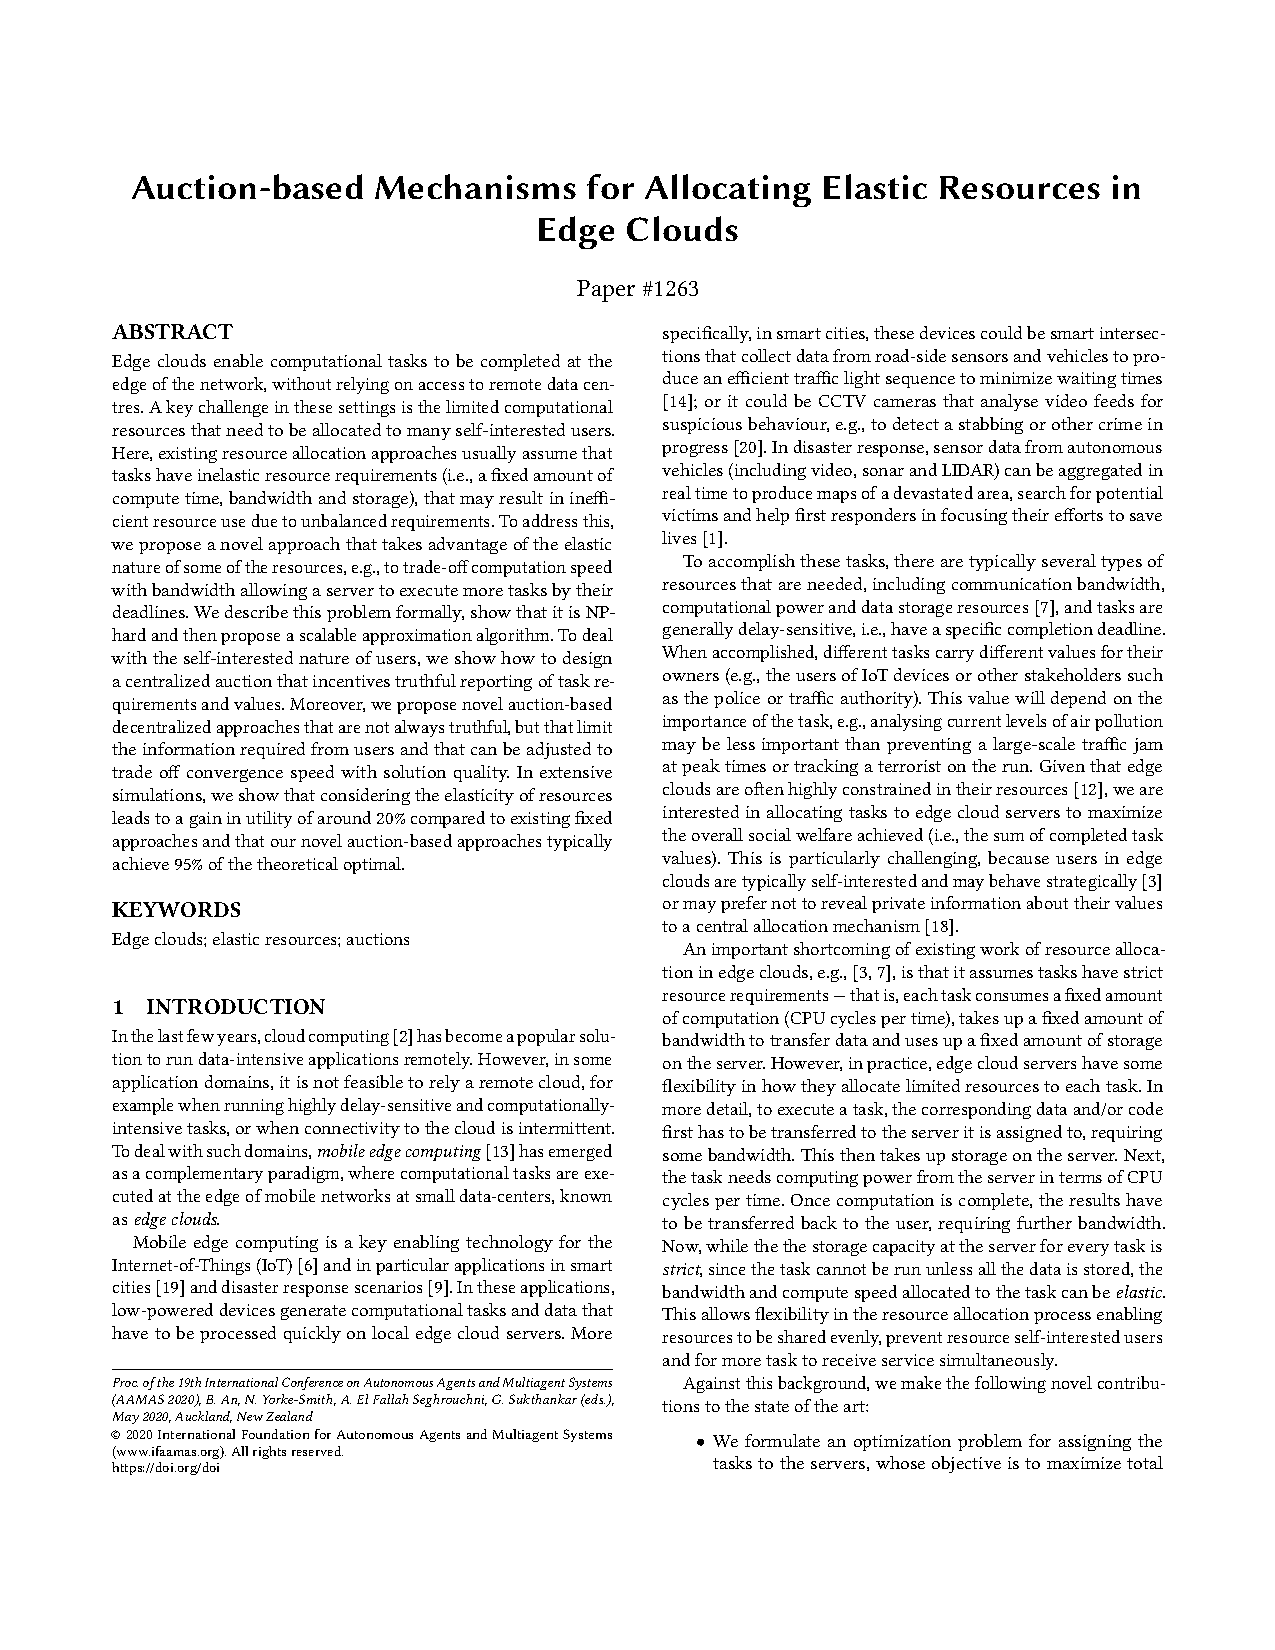
\includepdf[pages=-, offset=25mm -20mm]{extra/aamas_2020}

\section*{Appendix B: SPIE Presentation}
\label{app:spie-presentation}
The research of~\cite{FlexibleResourceAllocation} was presented at SPIE Defense + Commercial Sensing to the conference
on Artificial Intelligence and Machine Learning for Multi-Domain Operations Applications II under the title
"Analytical agility at the edge of the network through auction mechanisms".
\href{https://spie.org/SI/conferencedetails/artificial-intelligence-and-machine-learning-for-multi-domain-battle-applications#2560056}{Link}
to the recorded presentation.

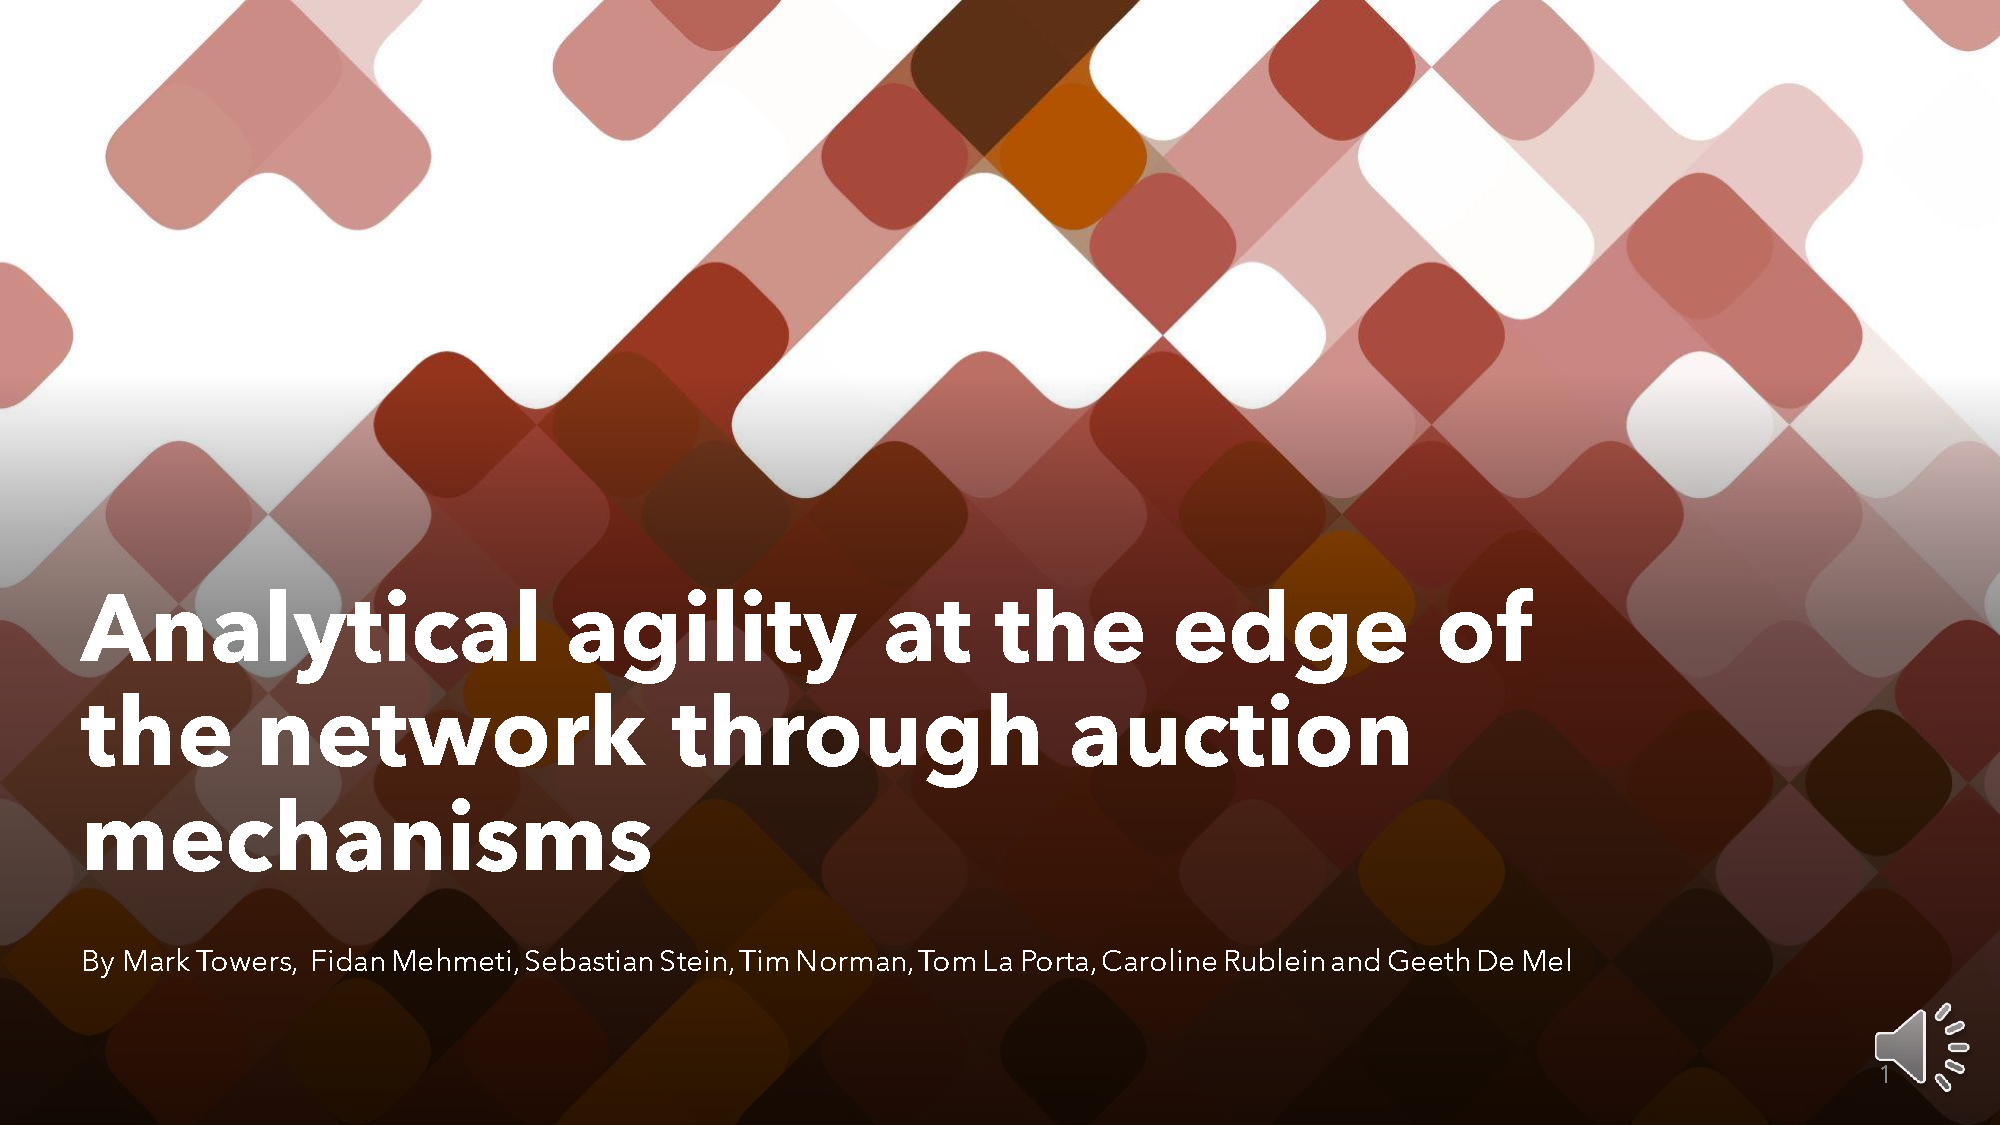
\includepdf[pages=-, offset=25mm -25mm, landscape=True, scale=0.95]{extra/spie_presentation}

\section*{Appendix C: Agent hyperparameters}
\label{app:agent-hyperparameters}
During training there are a range of hyperparameters for each agent, table~\ref{tab:agent_hyperparameters} provides
an explanation for the values for each hyperparameter used in the project.

\begin{longtable}{|p{2cm}|p{3.5cm}|p{2.5cm}|p{6cm}|} \hline
    \textbf{Agent} & \textbf{Properties name} & \textbf{Value} & \textbf{Explanation} \\ \hline
        RL Agent & batch\_size & 32 & The number of trajectories from the experience replay buffer that are used each
            time to train an agent. \\ \hline
        RL Agent & error\_loss\_fn & tf.losses. huber\_loss & The loss function used in calculating a network's error. \\ \hline
        RL Agent & initial\_training replay\_size & 5000 & The number of trajectories in the experience replay buffer
            required before the agent begins training. \\ \hline
        RL Agent & training\_freq & 2 & For every trajectory added to the experience replay buffer, for each 2, the
            agent tries to be trained. \\ \hline
        RL Agent & discount\_factor & 0.9 & Within the Q learning function (equation~\eqref{eq:q_learning}), the
            discount factor determines how important the rewards in the future impact the Q value. \\ \hline
        RL Agent & replay\_buffer length & 25000 & The length of the circular experience replay buffer. \\ \hline
        RL Agent & save\_frequency & 25000 & The agent networks are saved after 25000 time that agent has been trained
            \\ \hline
        RL Agent & training\_loss log\_freq & 250 & Tensorboard allows for data to be saved using training, after every
            the agent has been trained 250 time, the agents loss is logged for future analysis. \\ \hline
        Task Pricing RL Agent & reward\_scaling & 1 & \\ \hline
        Task Pricing RL Agent & failed\_auction reward & -0.05 & The reward for when the agent bids on a task but fails
            to win the auctioned task. \\ \hline
        Task Pricing RL Agent & failed\_multiplier & -1.5 & A multiplier applied to the winning price is the task fails
            to be computed within its deadline. \\ \hline
        Resource weighting RL Agent & other\_task\_discount & 0.4 & The multiplier to tasks not under consideration for
            a weighting action. \\ \hline
        Resource weighting RL Agent & success\_reward & 1 & The reward when the agent successfully completes a task
            \\ \hline
        Resource weighting RL Agent & failed\_reward & -1.5 & The reward when the agent fails to complete a task within
            its deadline. \\ \hline
        Dqn Agent & target\_update\_tau & 1.0 & The update tau value for use in the target update frequency. \\ \hline
        Dqn Agent & target\_update\_freq & 2500 & The target network in the DQN agent is updated after the agent
            has been updated 2500 times. \\ \hline
        Dqn Agent & initial\_epsilon & 1 & The initial exploration factor during training \\ \hline
        Dqn Agent & final\_epsilon & 0.1 & The final exploration factor during training \\ \hline
        Dqn Agent & epsilon\_steps & 10000 & The number of training step for linear exploration to move between the
            initial\_epsilon and the final\_epsilon factor. \\ \hline
        Dueling Dqn Agent & double\_loss & True & If to use the double dqn loss function \\ \hline
        Categorical Dqn Agent & max\_value & -20.0 & The maximum value for the value distribution \\ \hline
        Categorical Dqn Agent & min\_value & 25.0 & The minimum value for the value distribution \\ \hline
        Categorical Dqn Agent & num\_atoms & 21 & The number of atoms for each actions. \\ \hline
        Ddpg Agent & actor\_learning\_rate & 0.0001 & The learning rate for the optimiser for the actor network. \\ \hline
        Ddpg Agent & critic\_learning\_rate & 0.0005 & The learning rate for the optimiser for the critic network. \\ \hline
        Ddpg Agent & initial\_epsilon\_std & 0.8 & The initial exploration standard deviation of the normal distribution
            used  during training \\ \hline
        Ddpg Agent & final\_epsilon\_std & 0.05 & The final exploration standard deviation of the normal distribution
            used  during training \\ \hline
        Ddpg Agent & actor\_target update\_freq & 3000 & The actor target network update frequency \\ \hline
        Ddpg Agent & critic\_target update\_freq & 1500 & The critic target network update frequency \\ \hline
        Ddpg Agent & upper\_action bound & 30.0 & The upper action bound for the actor network \\ \hline
        Task pricing Ddpg Agent & min\_value & -100.0 & The minimum value for the critic network to estimate for an
            action \\ \hline
        Task pricing Ddpg Agent & max\_value & 100.0 & The maximum value for the critic network to estimate for an
            action\\ \hline
        Resource allocation Ddpg Agent & min\_value & -20 & The minimum value for the critic network to estimate for an
            action \\ \hline
        Resource allocation Ddpg Agent & max\_value & 15 & The maximum value for the critic network to estimate for an
            action\\ \hline
        TD3 Agent & actor\_update\_freq & 3 & The actor network update frequency for each critic network update. \\ \hline
    \caption{Agent hyperparameters}
    \label{tab:agent_hyperparameters}
\end{longtable}

\section*{Appendix D: Fixed Resource Allocation Optimisation Problem}
\label{app:fixed-resource-allocation-optimisation-problem}
Using the Flexible Resource Allocation Optimisation problem from Section~\ref{sec:resource-allocation-optimisation-problem},
to convert the problem to a Fixed Resource Allocation Optimisation problem requires two stages. \\
The first of these is to convert the flexible task specification to a fixed task specification, by solving the linear
programming equations~\ref{eq:fixed-task-objective} and~\ref{eq:fixed-task-deadline}. The equations forces the resource
usage speeds ($s^{'}_j$, $w^{'}_j$ and $r^{'}_j$) to be within the deadline (equation~\ref{eq:fixed-task-deadline}) and
that the objective function is to minimise the total resources used. The reason for speeds being raise to the power is
to prevent over use of a single resources (e.g. 5 loading speeds, 3 compute speed, 10 sending speed).

\begin{align}
    \text{min} & 1.2^{s^{'}_j} + 1.2^{w^{'}_j} + 1.2^{r^{'}_j} \label{eq:fixed-task-objective} \\
    \mbox{s.t.} \nonumber \\
    & \frac{s_j}{s^{'}_j} + \frac{w_j}{w^{'}_j} + \frac{r_j}{r^{'}_j} \leq d_j - a_j \label{eq:fixed-task-deadline} \\
\end{align}

The second stage is using the Fixed task specifications, to construct the server resource allocation optimisation
problem. The objective function (equation~\ref{eq:fixed-env-objective}) is to maximise the number of tasks that are
completed. The updated fixed tasks are denoted $J^{'}$. Due to there being a fixed resource allocation, the server
allocates all of the required resources over the tasks whole lifetime. As a result, the server computational and
bandwidth capacity constraints (equations~\ref{eq:fixed-server-computation-capacity}
and~\ref{eq:fixed-server-bandwidth-capacity}) allocates a task's resources over its whole lifetime. The server's storage
constraint is similar except with a task's storage increasing till the whole task's required storage is included.

\begin{align}
    \text{max} & \sum_{i \in I, j \in J^{'}} x_{i,j} \label{eq:fixed-env-objective} \\
    \mbox{s.t.} \nonumber \\
    & \sum_{\{j \in J^{'} | a_j \leq t \leq d_j\}} \text{min}(s_j, s^{'}_j \cdot (t + 1 - a_j)) \cdot x_{i,j} \leq S_i && \forall{i \in I} \label{eq:fixed-server-storage-capacity} \\
    & \sum_{\{j \in J^{'} | a_j \leq t \leq d_j\}} w^{'}_j x_{i,j} \leq W_i && \forall{i \in I} \label{eq:fixed-server-computation-capacity} \\
    & \sum_{\{j \in J^{'} | a_j \leq t \leq d_j\}} (s^{'}_j + r^{'}_j) \cdot x_{i,j} \leq R_i && \forall{i \in I} \label{eq:fixed-server-bandwidth-capacity} \\
    & \sum_{i \in I} x_{i,j} \leq 1 && \forall{j \in J^{'}} \label{eq:fixed-env-allocation-limit} \\
    & x_{i,j} \in \{0, 1\} && \forall{i \in I, j \in J^{'}} \label{eq:fixed-env-allocation-set}
\end{align}

\section*{Appendix E: Project management}
\label{app:project-management}
To management this project has been difficult due to having to split my time between writing the academic paper at the
start of the year (plus creating the recorded presentation) and the programming and write up the expanded research.
Because of this, a risk assessment (Table~\ref{tab:risk_assessment}) to understand possible risks during the project.
The project was also planned using a grantt chart (figure~\ref{fig:progress_grant_chart}) to understand the progress of
the project over time and to plan how the project would run. The project brief is submitted in October 2019
is included at the end of this report as well. The word count of the project generated by texcount for chapters 1 to 6
is included.

\subsection*{Risk assessment}
\begin{table}[H]
    \centering
    \begin{tabular}{|p{3cm}|c|c|p{7cm}|} \hline
        \textbf{Risk}  & \textbf{Severity} & \textbf{Possibility} & \textbf{Explanation} \\ \hline
        Rejected paper submission & 1 & 4 & The paper (Appendix A) was submitted to the AAMAS 2020 conference in
            December that could be rejected. While this was be disappointing if this happened, the paper can still be
            submitted to another conference at a later time. \\ \hline
        Iridis failure & 5 & 1 & In order to train the agent in this project, the University of Southampton supercomputer,
            Iridis 5 was utilised so if this could not be used anymore. This was cause massive issues to be able to
            train all of the agents for both long enough. \\ \hline
        Agent Training time & 4 & 2 & Reinforcement learning agents can take several million actions to achieve
            effective results which takes days or weeks to learn. This project doesn't have such resources or time to
            spend training agents to do this therefore making it a large problem. \\ \hline
        Personal Illness or Injury & 4 & 1 & Physical illness or injury could prevent the project from being both
            programmed or written. \\ \hline
        Pandemic & 4 & 1 & While Pandemic will not prevent the project from being completed due to all work being
            digital, it would prevent talking with my supervisor in person or for University to be open. \\ \hline
    \end{tabular}
    \caption{Risk Assessment}
    \label{tab:risk_assessment}
\end{table}

\subsection*{Progress Grantt Chart}
%% TODO compare project brief and progress report to actual report
\begin{figure}[H]
    \centering
    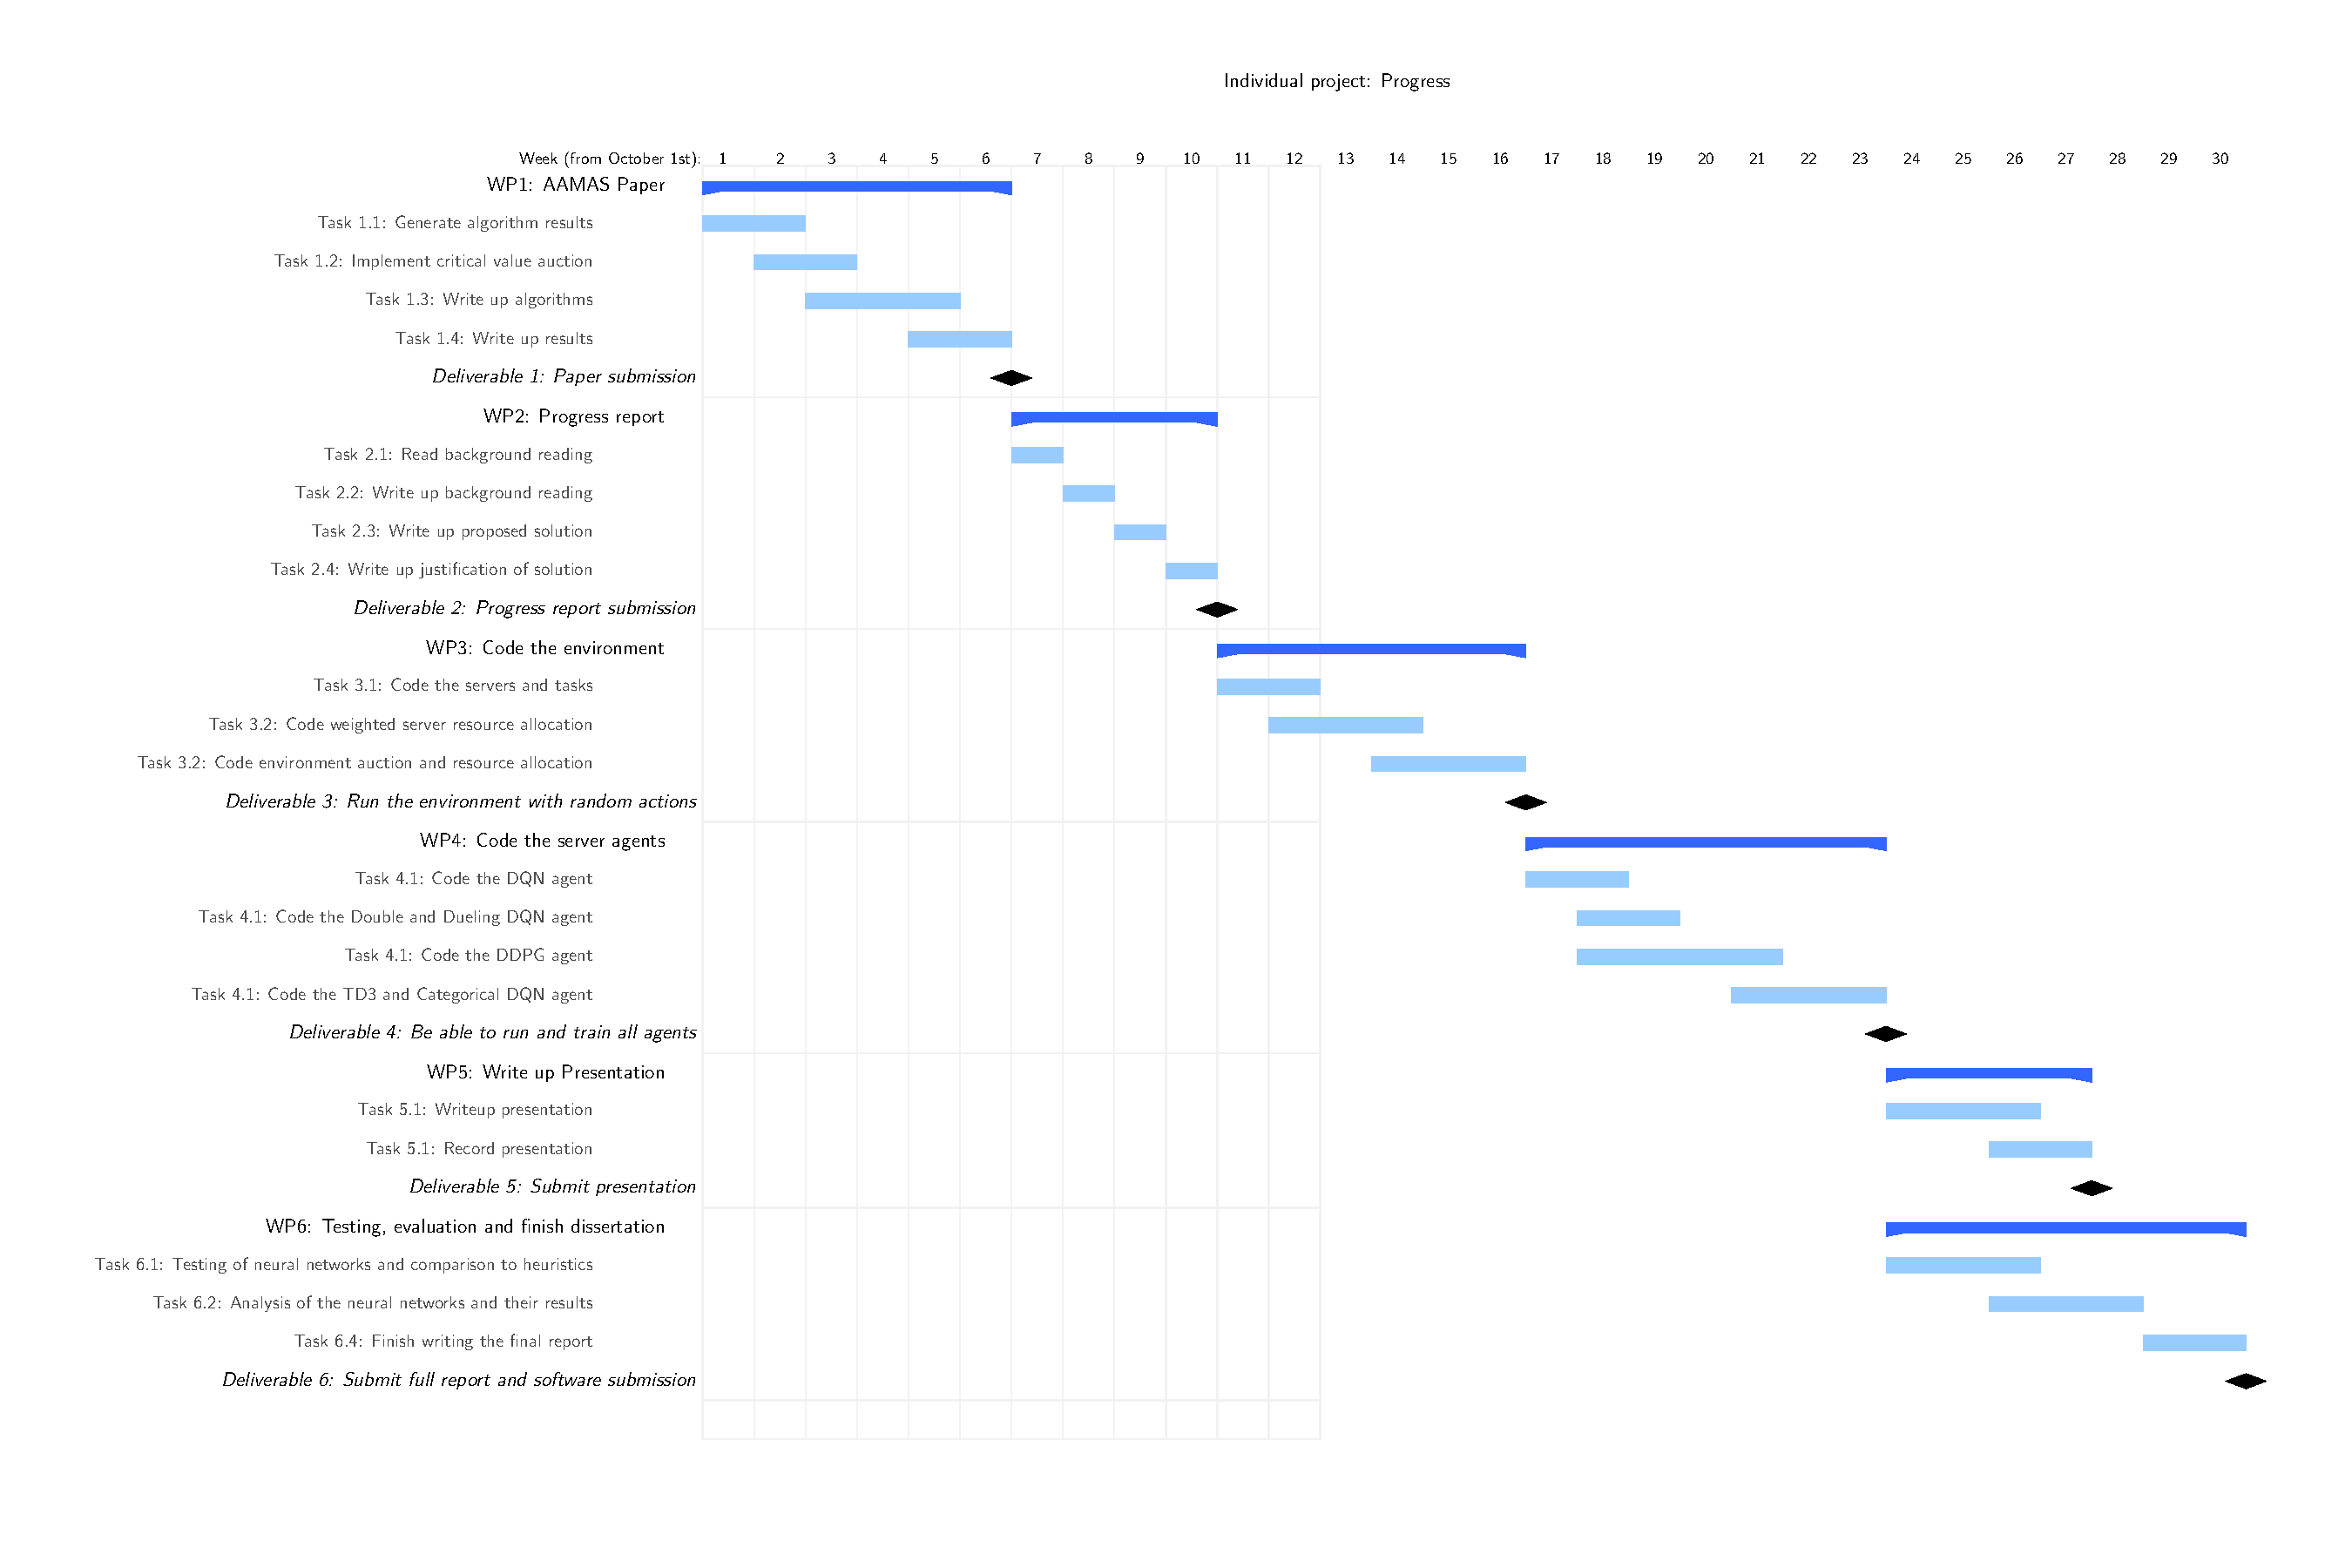
\includegraphics[width=\linewidth]{extra/progress_grantt_chart.pdf}
    \caption{Progress Grantt chart}
    \label{fig:progress_grant_chart}
\end{figure}

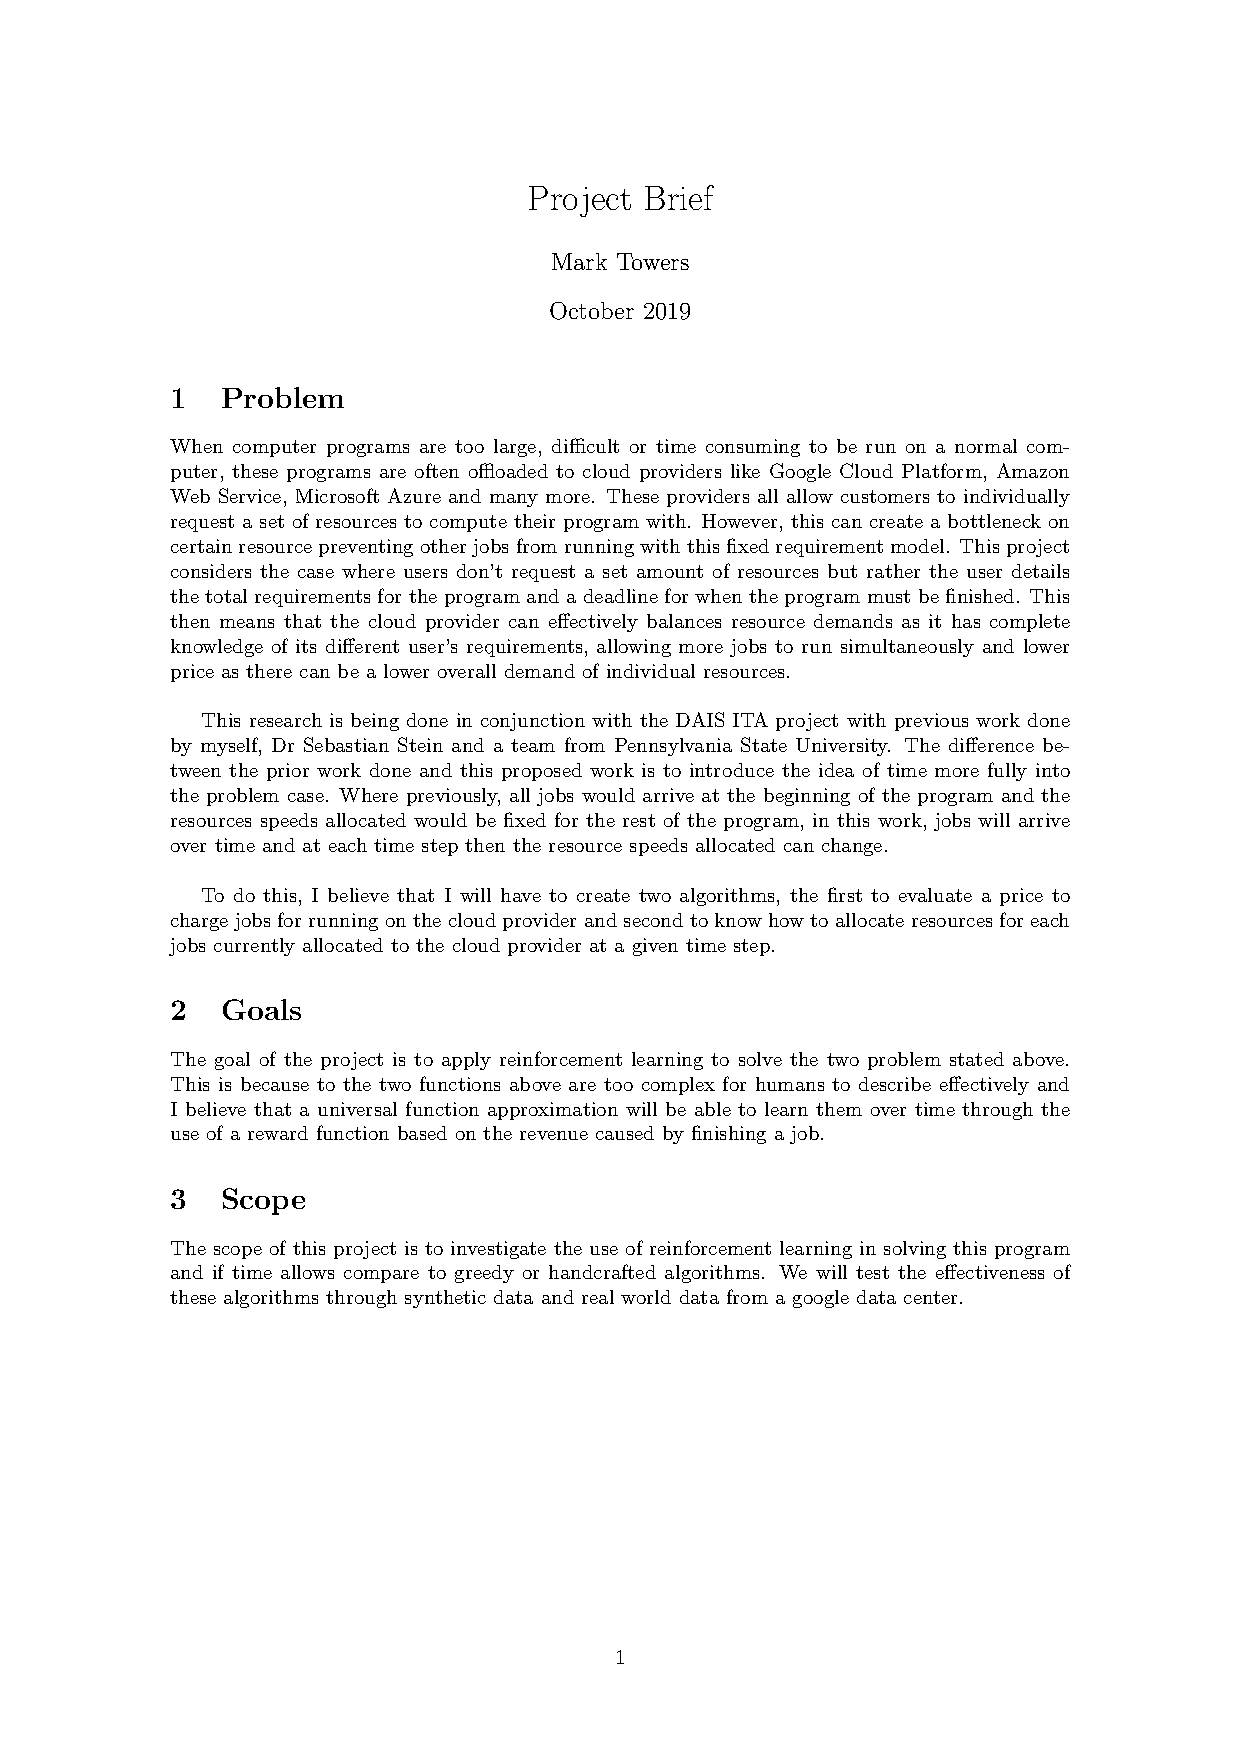
\includepdf[pages=-, offset=25mm -20mm]{extra/project_brief}

\subsection*{Word count}
% texcount -sum -inc chapters/1_introduction.tex chapters/2_background_lit.tex chapters/3_solution.tex chapters/4_implementation.tex chapters/5_evaluation.tex chapters/6_conclusion.tex -out=extra/wordcount.sum
\wordcount


\end{document}
%% ----------------------------------------------------------------
